\chapter{Rules with Data}
\label{chapter:early-violation-detection}
  
In this chapter, we address the problem of
detecting violations for rules with data.
Adding data variables over a data domain
expands the types of properties rules can express,
such as matching the user of a {\Payment} event
with the user who made the {\Request}.
First,
we consider the problem for an individual rule,
developing a technique for calculating the earliest time
a violation is inevitable (the ``deadline'')
and use this time for detecting violations of individual rules.
Then,
we observe that 
interactions within a set of rules
creates situations where
an enactment may violate a set of rules
though no individual rule is violated,
which is trivial in the absence of data
but non-trivial with data,
so we extend our algorithms to handle a set of rules
by simulating the effects of rule interaction using a chase process.
To ensure chase termination,
the chapter's results for multi-rule violation detection
are limited to ``acyclic'' sets of rules.
We also present two optimizations
to reduce computational overhead
of the violation detection algorithms.
Finally,
we evaluate the feasibility of our techniques
to determine where our approach is beneficial;
we implement the individual rule and multi-rule algorithms and
characterize their performance on a variety of enactments and rule sets.

This chapter is organized as follows.
Section\:\ref{sec:alg}
presents the {\sf Deadline} algorithm for computing deadlines,
then the data structures and 
{\sf Update}, {\sf Update-E}, {\sf Build}, and {\sf Detect} algorithms
for storing relevant event data
and detecting violations.
Section\:\ref{sec:multiple}
extends these techniques to 
acyclic sets of rules
with the {\sf Chase} and {\sf Detect-Multi} algorithms.
Section\:\ref{sec:opt}
presents two optimization techniques
for {\sf Update} and {\sf Update-E}.
Section\:\ref{sec:eval}
provides key findings of evaluations
of an implementation of the algorithms.
Finally,
Sections\:\ref{sec:early-violation-detection-related-work} and \ref{sec:rules-data-conclusion}
discuss related work and conclude the chapter.

\setlength{\tabcolsep}{0.2em} % for the horizontal padding
\renewcommand{\arraystretch}{1.2}% for the vertical padding
\long\def\BodyAssignNew{
\begin{figure}[t]
\centering
% \footnotesize
\vspace*{-1mm}
\begin{scriptsize}
\begin{tabular}[c]{c|c|c|c|c|c|c|l}\cline{2-7}
    \An{\tiny Aid}& \An{\tiny ID}  & \sps$u$ & \sps$a$ & \sps$x$   & \sps$y$   &  \sps$z$ &               \\\cline{2-7}
    \sps$\mu_{_1}$ & \sps$\pi_{_1}$ & \sAlice & \sps a3 & \sps 1    & \An{-}    & \An{-} &                              \\\cline{2-7}
    \sps$\mu_{_2}$ & \sps$\pi_{_1}$ & \sAlice & \sps a4 & \sps 3    & \An{-}    & \An{-} &                              \\\cline{2-7}
    \sps$\mu_{_3}$ & \sps$\pi_{_1}$ & \sAlice & \An{-}   & \An{-} & \sps 6 & \An{-} &                              \\\cline{2-7}
    \sps$\mu_{_4}$ & \sps$\pi_{_1}$ & \sAlice & \sps a3 & \sps 1 & \sps 6  & \An{-} & \sps$\mu_{_1} + \mu_{_3}$        \\\cline{2-7}
    \sps$\mu_{_5}$ & \sps$\pi_{_1}$ & \sAlice & \sps a4 & \sps 3 & \sps 6  & \An{-} & \sps$\mu_{_2} + \mu_{_3}$        \\\cline{2-7}
    \sps$\mu_{_6}$ & \sps$\pi_{_2}$ & \sBob   & \sps b6 & \sps 7 & \An{-}    & \An{-} &                              \\\cline{2-7}
    \sps$\mu_{_7}$ & \sps$\pi_{_1}$ & \sAlice & \sps a4 & \An{-} & \An{-}    & \sps 8  &                             \\\cline{2-7}
    \sps$\mu_{_8}$ & \sps$\pi_{_1}$ & \sAlice & \sps a4 & \sps 3 & \An{-}    & \sps 8  & \sps$\mu_{_2} + \mu_{_7}$     \\\cline{2-7}
    \sps$\mu_{_9}$ & \sps$\pi_{_1}$ & \sAlice & \sps a4 & \An{-} & \sps 6    & \sps 8  & \sps$\mu_{_3} + \mu_{_7}$     \\\cline{2-7}
    \sps$\mu_{_{10}}$ & \sps$\pi_{_1}$ & \sAlice & \sps a4 & \sps 3    & \sps 6 & \sps 8  & \sps$\mu_{_2} + \mu_{_{9}}$ \\\cline{2-7}
    \sps$\mu_{_{11}}$ & \sps$\pi_{_1}$ & \sAlice & \sps a3 & \An{-} & \An{-}    & \sps 9  &                            \\\cline{2-7}
    \sps$\mu_{_{12}}$ & \sps$\pi_{_1}$ & \sAlice & \sps a3 & \sps 1      & \An{-} & \sps 9  & \sps$\mu_{_{1}} + \mu_{_{11}}$ \\\cline{2-7}
    \sps$\mu_{_{13}}$ & \sps$\pi_{_1}$ & \sAlice & \sps a3 & \An{-} & \sps 6 & \sps 9  & \sps$\mu_{_{3}} + \mu_{_{11}}$  \\\cline{2-7}
    \sps$\mu_{_{14}}$ & \sps$\pi_{_1}$ & \sAlice & \sps a3 & \sps 1    & \sps 6 & \sps 9  & \sps$\mu_{_{4}} + \mu_{_{12}}$  \\\cline{2-7}
\end{tabular}
\hspace*{1mm}
\begin{tabular}[c]{c}
\begin{tabular}[c]{c|c|c|c|c|c|c|l}\cline{2-7}
  \An{\tiny Aid}   & \An{\tiny ID} & \sps$u$ & \sps$a$  & \sps$\,x\,$   & \sps$y$  & \sps$z$  &                            \\\cline{2-7}
  \sps$\mu_{_{15}}$ & \sps$\pi_{_1}$ & \sAlice &\An{-} & \An{-} & \sps 10 & \An{-} &                           \\\cline{2-7}
  \sps$\mu_{_{16}}$ & \sps$\pi_{_1}$ & \sAlice & \sps a4 & \sps 3 & \sps 10  & \An{-} & \sps$\mu_{_2} + \mu_{_{15}}$  \\\cline{2-7}
  \sps$\mu_{_{17}}$ & \sps$\pi_{_2}$ & \sBob   & \An{-}  &   \An{-}  & \sps 10  & \An{-}                             \\\cline{2-7}
  \sps$\mu_{_{18}}$ & \sps$\pi_{_2}$ & \sBob   & \sps b6 & \sps 7 & \sps 10  & \An{-} & \sps$\mu_{_6} + \mu_{_{17}}$   \\\cline{2-7}
\end{tabular}
\\\mbox{~}\\*[-1mm]
  \footnotesize
  (b) New body assignments added at time $10$
\end{tabular}
\\*[3pt]
\end{scriptsize}
\hspace*{14mm}
{\footnotesize(a) All body assignments at time 9\hfill}
\caption{Assignments for the rule body $\varphi$ and events $S_{_9}$, events $S_{_9}{\cup}\{e_1,e_2\}$}
\label{fig:example_assignments}
\end{figure}
} 

\setlength{\tabcolsep}{0.2em}
{\renewcommand{\arraystretch}{1.2}}
\long\def\BodyTableExample{
\begin{tabular}[c]{|c|c|c|c|c|c|c|c|}\cline{1-8}
  \An{\tiny Aid}  & \sps$u$ & \sps$a$ & \sps$x$ & \sps$y$ & \sps$z$  & \sps gap atoms  & \sps match?   \\\cline{1-8}
  \sps$\mu_{_{10}}$ & \sAlice & \sps a4 & \sps 3 & \sps 6 & \sps 8 &  $\An{-}$  & \sps No       \\\cline{1-8} 
  \sps$\mu_{_{11}}$ & \sAlice & \sps a3 & \An{-} & \An{-} & \sps 9 & \sps$x{\leq}y{\leq}x{+}7,$& \sps No       \\*[-4pt]
    & & & & & & \sps$y{\leq}9{\leq}y{+}7$ &   \\\cline{1-8}
  \sps$\mu_{_{12}}$ & \sAlice & \sps a3 & \sps 1 & \An{-} & \sps 9 & \sps$1{\leq}y{\leq}8,$    & \sps No \\*[-4pt]
    & & & & & & \sps$y{\leq}9{\leq}y{+}7$ &   \\\cline{1-8}
  \sps$\mu_{_{13}}$ & \sAlice & \sps a3 & \An{-} & \sps 6 & \sps 9 & \sps$x{\leq}6{\leq}x{+}7$ & \sps No  \\\cline{1-8}
  \sps$\mu_{_{14}}$  & \sAlice & \sps a3 & \sps 1 & \sps 6 & \sps 9 &  $\An{-}$    & \sps No  \\\cline{1-8}
\end{tabular}\smallskip
}
\long\def\HeadTableExample{
\begin{tabular}[c]{|c|c|c|c|c|c|}\cline{1-6}
  \An{\tiny Aid} & \sps$u$ & \sps$a$  & \sps$w$ & \sps$v$ & \sps gap atoms  \\\cline{1-6}
  \sps$\beta_{_{1}}$ & \sAlice & \sps a3 & \sps 8 & \An{-}  & \sps$v{\leq}12$  \\\cline{1-6}
  \sps$\beta_{_{2}}$ & \sAlice & \sps a4 & \sps 9 & \An{-}  & \sps$v{\leq}13$  \\\cline{1-6}
  \sps$\beta_{_{3}}$ & \sAlice & \sps a3 & \An{-} & \sps 12 & \sps$8{\leq}w$  \\\cline{1-6}
  \sps$\beta_{_{4}}$ & \sAlice & \sps a3 & \sps 8 & \sps 10 & \An{-}  \\\cline{1-6}
\end{tabular}\smallskip
}

\long\def\BodyHeadTables{
\begin{figure}[ht]
\centering
\begin{scriptsize}
\begin{tabular}[c]{c}
  \BodyTableExample\\\scriptsize
  (a) Some assignments in $\BODY/_r(\pi_{1})$ (Fig.\ref{fig:example_assignments}(a)) at $\tmsp=9$
\end{tabular}
\begin{tabular}[c]{c}
  \HeadTableExample \\\scriptsize
  (b) Some assignments in $\HEAD/_r(\pi{_1})$ (Fig.\ref{fig:example_assignments}(b)) at $\tmsp=10$
\end{tabular}
\end{scriptsize}
\vspace*{-2mm}
\caption{Body and Head Table Examples}
\label{fig:BodyHeadTables}
\end{figure}  
}

\long\def\BodyTable{
\begin{figure}[ht]
\centering\footnotesize
\vspace*{-3mm}
\begin{scriptsize}
  \BodyTableExample
\end{scriptsize}
\vspace*{-2mm}
\caption{Some assignments in $\BODY/_r(\pi_{1})$ at $\tmsp=10$ (Fig.\ref{fig:example_assignments})}
\label{fig:BodyTable}
\end{figure}  
}
\long\def\HeadTable{
\begin{figure}[ht]
\centering\footnotesize
\vspace*{-3mm}
\begin{scriptsize}
  \HeadTableExample
\end{scriptsize}
\vspace*{-2mm}
\caption{Assignments in $\HEAD/_r(\pi_{1})$ at $\tmsp=15$}
\label{fig:HeadTable}
\end{figure}  
}

\long\def\ExtensionTable{
\begin{figure}[ht]
\centering
\vspace*{-2mm}
\begin{scriptsize}
\begin{tabular}[c]{|c|c|c|}
  \cline{1-3}
  \sps body \An{\tiny Aid}  & \sps head \An{\tiny Aid} & \sps deadline   \\\cline{1-3}
  \sps$\mu_{_{10}}$  &  $\An{-}$  & \sps 9        \\\cline{1-3}
  \sps$\mu_{_{10}}$  &  \sps$\beta_2$ & \sps 13   \\\cline{1-3}
  \sps$\mu_{_{14}}$  &  $\An{-}$  & \sps 9        \\\cline{1-3}
  \sps$\mu_{_{14}}$  &  \sps$\beta_1$ & \sps 12   \\\cline{1-3}
  \sps$\mu_{_{14}}$  &  \sps$\beta_3$ & \sps 12   \\\cline{1-3}
  \sps$\mu_{_{14}}$  &  \sps$\beta_4$ & $\An{-}$  \\\cline{1-3}
\end{tabular}\\*[3pt]
\end{scriptsize}
\vspace*{-2mm}
\caption{Extensions of $\mu_{_{10}}$ and $\mu_{_{14}}$ in $\EXT_r(\pi_{1})$ at $\tmsp=13$}
\label{fig:ExtensionTable}
\end{figure}  
}

\section{Algorithms for Individual Rules}
\label{sec:alg}

In this section,
we develop key techniques for
early violation detection for individual rules.
First,
we define the concept of deadlines
and present an algorithm to calculate deadlines.
We then define data structures
to store variable assignments and
present algorithms
to create new assignments from arriving events,
and to merge and match existing assignments.
Finally,
we detail how violations are detected
using these algorithms.

\smallskip

We aim to detect violations
at the earliest possible time.
Since an enactment is an accumulation of
events with increasing timestamps,
it may be that
a complete body assignment derived
from the current enactment
can only be extended
at or before a specific future time
called a deadline.
We now formulate the notion of a deadline below.

\begin{deff}
  Let $\Theta$ be a set of gap atoms over variables
  $\seq{x}{n}$ and $\mu$ an assignment for variables $x_i$'s.
  We use {\sc def}$_{\!\mu}$ for the
  variables $\mu$ assigns a value;
  $\mu(\Theta)$ the gap atoms obtained
  % from $\Theta$
  by replacing each variable $x\tight\in \textsc{def}_{\!\mu}$
  with $\mu(x)$,
  and $\max(\mu)\tight=\max\{\mu(x)\tight| x\in \textsc{def}_{\!\mu}\}$.
  A timestamp $\tau\tight\in\N$ is
  the {\em deadline} for $\Theta, \seq{x}{n}, \mu$
  if
  (1) $\tau{\ge}\max(\mu)$,
  and
  (2) either
  $\mu(\Theta)$ is unsatisfiable and $\tau{=}\max(\mu)$
  or
  conditions (i) and (ii) both hold:
  (i) for each complete extension $\mu'$ of $\mu$
  such that
  $\mu'(x)\tight>\tau$ for each $x\tight\notin\textsc{def}_{\!\mu}$,
  $\mu'(\Theta)$ is {\sl false}, and
  (ii) there is a complete extension $\mu''$ of $\mu$
  such that $\mu''(\Theta)$ is {\sl true}.
\end{deff}

\begin{figure}[ht]
  \centering
  {\StateS9}
  \caption{\normalsize Database $S_{_9}$ with events from two enactments $\pi_1$ and $\pi_2$.}
  \label{fig:example_state}
\end{figure}

\begin{figure}[!ht]
\begin{center}
  \vspace*{-2mm}
~~~~~~~~~$r_1:\ \Request(u,a)@x,
\Approval(u)@y,
x {\leq} y {\leq} x {+} 7,
\Reserve(u,a)@z,
y {\leq} z {\leq}$ $y{+}7$\\
$\rightarrow
\Payment(u,a)@w,
\Launch(u,a)@v,
y{\le} w {\leq} y {+} 3,
z{\le} v {\leq} z {+} 7,
v{\leq}w+4$
\vspace*{-2mm}
\end{center}
\caption{Rule $r_1$}
\label{fig:example_rule_r_1}
\end{figure}

\begin{examp}
  For the example enactment introduced in Section\:\ref{sec:motiv}
  and rule $r_1$ in Fig.\:\ref{fig:example_rule_r_1},
  the body assignment $\mu_{_{10}\!}$ is created at time $8$,
  where $\mu_{_{10}\!}(x){=}3$,
  $\mu_{_{10}\!}(y){=}6$, and
  $\mu_{_{10}\!}({z}){=}8$.
  As shown in Fig.\:\ref{fig:example_deadline_minimum},
  applying $\mu_{_{10}\!}$ to the head atoms
  yields upper bounds $w\tight\leq 9$ (${=}y{+}3)$ and
  $v\tight\leq 15$ (${=}{z}{+}7$).
  These bounds show that extensions of $\mu_{_{10}}$
  must have a {\Payment} event whose time variable $w$
  is no later than time $9$.
  Thus, the time $9$ is a {\em deadline} for $\mu_{_{10}}$:
  the latest time $\mu_{_{10}}$ can be extended w.r.t. $w$,
  and the earliest time $\mu_{_{10}}$ 
  could be recognized as a witness of a violation.
  Fortunately,
  a {\Payment} event happened at time $9$,
  which satisfies $w\tight\leq 9$.
  However,
  $v$ remains unresolved and thus
  the subsequent deadline to extend $\mu_{_{10}}$ is
  the latest time to observe a value for $v$:
  $v\tight\leq 13$ (${=}{w}{+}4$)
  and 
  $v\tight\leq 15$ (${=}{z}{+}7$),
  so the deadline to extend $\mu_{_{10}}$ is changed to $13$.
\end{examp}

\begin{algorithm}[t]
\caption{{\sf Deadline}$(\Theta,\seq{x}{n},\mu)$}
\label{alg:deadline}
\begin{small}\vspace*{-2.5mm}
\begin{flushleft}
  \algorithmicrequire{
    A set of gap atoms $\Theta$ over
    time variables $\seq{x}{n}$ and an assignment $\mu$}
  \\
  \algorithmicensure{ A timestamp $\tau$}
  \end{flushleft}\vspace*{-3.5mm}
  \begin{algorithmic}[1]
    \If{If $\mu(\Theta)$ is unsatisfiable}
    {\bf return} $\tau := \max(\mu)$;\vspace*{-2pt}\newline\mbox{~}\hfill
    /$*$ $\max(\mu)$ is the largest timestamp $\mu$ assigns to $\seq{x}{n}$$*$/
  \EndIf{}
  \State{Rewrite each atom in $\mu(\Theta)$ in the form $u\tight\pm k\tight\leq v$;
    \vspace*{-2pt}\newline\hspace*{1cm}
    \hfill
    /$*$ $u,v$ either a time variable or in $\N$, $k\tight\in\Z$  $*$/}
  \State{Let \textsl{UpperBd} be a map from $\seq{x}{n}$ to $\{\infty\}$;}
  \For{each $u\tight{\pm}k\tight\le v$ in $\mu(\Theta)$
      with $v\tight\in\N$ and $u\tight\in \{\seq{x}{n}\}$}
    \State{$\textsl{UpperBd}(u) := v\tight{\mp}k$\:;}
  \EndFor
  \For{$|\Theta|$ iterations}
    \For{each gap atom $u\tight{\pm}k\tight\leq v$ in $\mu(\Theta)$}
      \If{$\textsl{UpperBd}(v)$ is finite and $\textsl{UpperBd}(u)\tight{\pm}k\tight>
          \textsl{UpperBd}(v)\tight\geq 0$}
        \State{$\textsl{UpperBd}(u) := \textsl{UpperBd}(v)\tight{\mp}k$\:;}
      \EndIf
    \EndFor
  \EndFor
  \State{{\bf return} $\tau:=\min\{\textsl{UpperBd}(x_i)\tight\mid 1{\le}i{\le}n\}$}
  \end{algorithmic}
\end{small}
\end{algorithm}  

We compute deadlines with function {\sf Deadline} (Alg.\:\ref{alg:deadline}).
{\sf Deadline}
determines
for each $x_i$ the least $\tau_i$ such that 
$\mu(\Theta)
\tight\rightarrow 
x_i{\leq}\tau_i$,
and
the deadline $\tau$ is the least of $\tau_i$'s.
First, if $\mu(\Theta)$ is unsatisfiable,
$\mu$ is a violation
at the time of its creation,
i.e., at its largest timestamp.
Otherwise,
an array \textsl{UpperBd} is initialized
with constants (Lines 3-5),
then tightened
with the initial bounds
and the gap atoms in $\Theta$:
a gap atom $u\tight\pm k\tight\leq v$
indicates $\textsl{UpperBd}(v)\tight\mp k$ is an upper bound for $u$.
For each gap atom $u\tight\pm k\tight\leq v$
for which $\textsl{UpperBd}(v)$ is defined,
we update
$\textsl{UpperBd}(u)$ as $\max(\textsl{UpperBd}(v)\tight\mp k,
\textsl{UpperBd}(u))$
(Lines 7-9).

\def\DDL{\textsf{Deadline}}

The {\DDL} function (Alg.\:\ref{alg:deadline})
can compute deadlines for complete body assignments
and for complete body assignments with matching partial head assignments.
For a complete body assignment $\mu$
and a partial head assignment $\beta$,
we compute the latest time $\mu\tight\cup\beta$ can be extended.
This time is, in fact,
the earliest time $\mu$ becomes a witness for a violation.
In the following lemma,
we state a property of deadlines
for a complete body assignment
and partial head assignment.

\begin{lemma}\label{lemma:deadline}
  Let $r{:}\:\varphi{\rightarrow}\psi$ be a rule,
  $\varphi_g,\psi_g$ the gap atoms in $\varphi,\psi$ (resp.),
  $\mu$ a (body) assignment such that $\mu(\varphi_g)$ is {\sl true},
  $\beta$ an incomplete head assignment matching $\mu$
  such that $\beta(\mu(\psi_g))$ is satisfiable,
  and
  $U$ the variables in $\psi_g$ undefined by $\beta$.
  Let\\
  $\tau\tight={\sf Deadline}(\psi_g,\var(\varphi_g\tight\cup\psi_g),\mu\tight\cup\beta)$.
  The following hold:
  \begin{enumerate}
  \item If $\tau\tight\in\N$,
    then there is a head assignment $\beta'$ matching
    $\mu\tight\cup\beta$
    such that $\min(\beta'(U))\tight\leq\tau$ and $\beta'(\psi_g)$ is
    {\sl true},
  \item If $\tau\tight\in\N$,
    then for all complete head assignments $\beta'$ matching
    $\mu\tight\cup\beta$
    such that

    $\max(\beta'(U)){>}\tau$, $\beta'(\psi_g)$
    is {\sl false}, and
  \item
    If $\tau=\infty$,
    then for all timestamps $n$ in $\N$,
    there is a head assignment $\beta'$ matching $\mu\tight\cup\beta$
    such that $\max(\beta'(U))\tight>n$ and $\beta'(\psi_g)$
    is {\sl true}. 
  \end{enumerate}
\end{lemma}

\begin{proof}
  To show (1),
  assume there is no complete head assignment $\beta'$
  extending $\mu\tight\cup\beta$
  such that $\min(\beta'(U))\tight\leq\tau$
  and $\beta'(\psi_g)$ is {\sl true}.
  Then,
  $(\mu\cup\beta)(\psi)\land (z=\tau)$
  is not satisfiable.
  Then,
  there is a gap atom in $\mu\cup\beta(\psi)$
  that provides an upper bound for $z$
  below $\tau$.
  Then,
  $\tau$ is not the minimum of the upper bounds
  in $\textsl{UpperBd}$.
  Thus Algorithm\:\ref{alg:deadline}
  on $\mu\cup\beta$ and $\psi$ should not output $\tau$.
  This is a contradiction.
  To show (2), assume some complete head assignment $\beta'$
  extends $\mu\tight\cup\beta$
  such that $\min(\beta'(U))\tight>\tau$
  and $\beta'(\psi_g)$ is true.
  Then, 
  $(\mu\cup\beta)(\psi)\land (z=\tau')$
  is satisfiable for some $z$ in $\var(\psi)$.
  Then, $\mu(\psi)$ does not imply $z_i\leq \tau$
  for all variables $z_i$.
  Thus Algorithm\:\ref{alg:deadline}
  on $\mu\cup\beta$ and $\psi$ should not output $\tau$.
  This is a contradiction.
  To show (3),
  assume $\tau=\infty$.
  Algorithm\:\ref{alg:deadline} only produces 
  $\infty$ when
  $\mu(\psi)$ is satisfiable and 
  for some variable $z_i$ and for all $n\in\N$,
  $\mu(\psi)\not\rightarrow (z_i \leq n)$
  Then,
  for all timestamps $n$ in $\N$,
  there is some complete assignment that extends $\mu$,
  satisfies $\psi$,
  and uses some $n'$ larger than $n$.
  Finally,
  $\mu$ can be extended arbitrary far in the future.
\end{proof}

The discussions in Section\:\ref{sec:motiv}
suggest
maintaining partial and complete assignments for rule variables.
We define three tabular data structures:
$\BODY/_r$ for body assignments,
$\HEAD/_r$ for head assignments, and
$\EXT_r$ (extensions),
to track pairings of body and head assignments.
$\BODY/_r$ and $\HEAD/_r$ consist of the following columns:
(\!{\em i}) one column for the assignment identifier ({\it Aid}) from $\ID$,
(\!{\em ii}) one column for the enactment identifier ({\sc id}) from $\ID$,
(\!{\em iii}) one column in $\BODY/_r$ for each variable in $\varphi$ and
one column in $\HEAD/_r$ for each event variable in $\psi$ (resp.)
(a variable in the head $\psi$ is an {\em event variable}
if it occurs in an event atom in $\psi$.)
to hold a value from $\Dom$ or a timestamp, and
(\!{\em iv}) one column for gap atoms in $\varphi$ and $\psi$ (resp.)
simplified with the assigned values as possible.
Additionally,
$\BODY/_r$ has one more column
(\!{\em v}) {\em match?} indicating with {\em yes} or {\em no}
the presence or absence, resp.,
of a complete head assignment matching the complete body assignment.
For convenience, we refer to rows in these two tables as assignments.
$\EXT_r$ has three columns:
(\!{\em i}) one column for a body {\it Aid} from $\BODY/_r$,
(\!{\em ii}) one column for a head {\it Aid} from $\HEAD/_r$
that extends the row's body assignment, 
and 
(\!{\em iii}) one column for the {\em deadline},
calculated using the row's assignments and the head gap atoms
as inputs for ${\sf Deadline}$.

For each enactment $\eta$,
$\BODY/_r(\eta)$ and $\HEAD/_r(\eta)$
store all assignments
that can be generated from set of events in $\eta$
and
satisfy $\varphi$ and $\psi$ (resp.).
Specifically,
for a rule $r{:}\:\varphi\tight\rightarrow\psi$
and an enactment $\eta$,
$\BODY/_r(\eta)$ contains every assignment $\mu$ such that
for a non-empty subset $P$ of the event atoms in $\varphi$,
$\mu$ is defined for the variables in $P$,
$\mu(P)\tight\subseteq \eta$,
and 
for each gap atom $g$ whose variables appear in $P$, 
$\eta$ satisfies $g$ with $\mu$.
$\HEAD/_r(\eta)$ is similar, using $\psi$ instead of $\varphi$.
Fig.\:\ref{fig:BodyHeadTables}(a)
shows the assignments inserted into $\BODY/_r$ table
at time $10$ (those from Fig.\:\ref{fig:example_assignments}(b))
with columns for gap atoms and the possibility of matching.
$\EXT_r(\eta)$ stores each pair of assignments
from $\BODY/_r(\eta)$ and $\HEAD/_r(\eta)$, resp.,
such that the body assignment can be extended
by the head assignment
only at or before the row's deadline,
i.e., some unknown variable in the body and head assignments
is constrained by a gap atom in the body or head
to be at or before the deadline.

{\BodyAssignNew}

\begin{examp}\label{e-update}
Given the events up to time $9$ in Fig.\:\ref{fig:example_state},
suppose two events happen at time $10$,
$e_1{:}\Approval(\pi_{_1\!},[\mbox{Alice}],10)$
and
$e_2{:}\Approval(\pi_{_2\!},[\mbox{Bob}],10)$.
Event $e_1$ generates an assignment
$\mu_{_{16}}{:}\,[\pi_{_1}\!,\allowbreak\mbox{Alice},\mbox{-},\mbox{-},10,\mbox{-}]$,
which combines with $\mu_{_2}$ into $\mu_{_{16}}$.
Event $e_2$ yields
new assignments
$\mu_{_{17}}$
and
$\mu_{_{18}}$.
Fig.\,\ref{fig:example_assignments}(b)
lists four assignments generated by $e_1$ and $e_2$.
\end{examp}

{\BodyHeadTables}

{\ExtensionTable}

We next present the {\sf Update} algorithm
to create and combine assignments
with a batch of events,
as shown in Example\:\ref{e-update}.
This algorithm maintains
$\BODY/$ and $\HEAD/$ incrementally
without accessing the corresponding enactment directly;
this is important
since enactments may be very large.



\begin{algorithm}[t]
\caption{{\sf Update}$(\Theta, \Delta, T(\eta))$}
\label{alg:update_assmt_table}
\begin{small}\vspace*{-2.5mm}
\begin{flushleft}
  \algorithmicrequire{
    A set of atoms $\Theta$,
    a batch $\Delta$ for an enactment $\eta$,
    a table $T(\eta)$ ($T$ is $\BODY/_r$ or $\HEAD/_r$)}\\
  \algorithmicensure{ The updated table $T(\eta\tight\cup\Delta)$ for $\eta\tight\cup\Delta$}
\end{flushleft}\vspace*{-3.5mm}
\begin{algorithmic}[1]
  \State{$\Gamma:= T(\eta)$\:;}
  \For{each event $e\in\Delta$}
    \For{each event atom $\gamma$ in $\Theta$ with the same name as $e$}
      \State{Create an assignment $\mu$ such that $\mu(\gamma)=e$\:;}
      \If{$\mu(\Theta)$ is satisfiable}
        \State{Add to $\Gamma$ the row
        $s=\langle a, e.\textsc{id}, \mu(v_1), ...,\mu(v_n),\textsc{b},(\An{no})\rangle$,\vspace*{-2pt}
        \newline\hspace*{4.0em}where $a$ is a fresh assignment identifier,
        $v_1,...,v_n$ are the event variables\vspace*{-2pt}
        \newline\hspace*{4.0em}in $\Theta$, and
        $\textsc{b}$ the gap atoms in $\Theta$, evaluated and simplified with $\mu$;}
      \EndIf
    \EndFor
  \EndFor
  \While{$\Gamma$ {\sl changes}}
  \For{each pair of unique and {\em consistent} rows $\mu_1$ and $\mu_2$ in $T$}
  \State{$\mu:=$\textit{merge}$(\mu_1, \mu_2)$\:;\hfill /$*$ {\em consistent}, {\em merge} explained in the text $*$/}
    \If{$\mu(\Theta)$ is satisfiable}
      \State {Add to $\Gamma$ the row:
      $s=\langle a, \mu_1.\textsc{id}, \max(t_1,t_2), \mu(v_1), ...,\mu(v_n), \textsc{b},(\An{no})\rangle$
      \vspace*{-2pt}
      \newline\hspace*{3.0em}where $a$ is a fresh assignment identifier and
      \vspace*{-2pt}
      \newline\hspace*{3.0em}$\textsc{b}$ is the union of gap atoms in $\mu_1,\mu_2$, evaluated with $\mu$\:;}
    \EndIf
  \EndFor
  \EndWhile
  \State{{\bf output} $\Gamma$}
  \end{algorithmic}
\end{small}
\end{algorithm}

We now outline the behavior of {\sf Update}.
Given atoms $\Theta$ (here, the body or head of a rule),
a batch $\Delta$,
and either $\BODY/_r$ or $\HEAD/_r$ for an enactment $\eta$,
First,
the events in $\Delta$ and $\Theta$ are used to generate assignments,
which are added to the table
if they are consistent with $\Theta$'s gap atoms,
(and thus extendible to complete assignments).
Then, the {\bf while} loop searches for
pairs of consistent, partial assignments;
two assignments are consistent if they agree
on the variables for which they are both defined,
e.g., in Fig.\:\ref{fig:example_assignments}
$\mu_{_1\!}$ and $\mu_{_2\!}$ agree on $u$ but not on $a$,
so they are not consistent.
For each pair of consistent assignments,
a new assignment is created
by combining their variable mappings and gap atoms
and a deadline is computed.
For example, assignment $\mu_{_5\!}$ in Fig.\:\ref{fig:example_assignments}
is the {\em merge} of $\mu_{_2\!}$ and $\mu_{_3\!}$.
If the new assignment is consistent with $\Theta$,
it is added to the table.
The {\bf while} loop considers only pairs of assignments
pre-existing in $\Gamma$ or $\Delta$,
i.e., it doesn't introduce new data values;
this ensures that {\bf while} loop terminates.

\begin{examp}
  For the enactment and rule in Section\:\ref{sec:motiv},
  consider the enactment's event
  $\Request(\pi_{_1\!}, [\mbox{Alice}, \mbox{a3}],1)$
  and the rule's atom
  $\Request(\mbox{user}\:u, \mbox{account}\:a)@x$.
  The mapping
  $[{\eid}\tight\mapsto \pi_{_1\!},\allowbreak
  u\tight\mapsto \mbox{Alice},\allowbreak
  v\tight\mapsto \mbox{a3},\allowbreak
  x\tight\mapsto 1]$
  maps the atom to this event;
  the assignment
  corresponding to this mapping
  is added to $\BODY/_r$
  as $\mu_{_1\!}$ in
  Fig.\:\ref{fig:example_assignments}(a).
  For the same example in Section\:\ref{sec:motiv}
  and Fig.\:\ref{fig:example_assignments}(a),
  assignments $\mu_{_2}{:}\:$
  [$\pi_{_1\!},\mbox{Alice},$
  $\mbox{a4}, 3, -, -,$
  $\{3{\leq}y{\leq}10, y{\leq} {z}{\leq} y{+}7\}$]
  and
  $\mu_{_3}{:}\:
  [\pi_{_1\!}, \mbox{Alice}, -, -, 6, -,
  \{x {\leq} 6{\leq} x{+}7,$ 
  $6{\leq} {z}{\leq} 13\}$]
  are in $\BODY/_r(\pi_{1})$ at $\tmsp=9$
  and agree on $u$.
  Their combination $\textit{merge}(\mu_{_2\!},\mu_{_3\!})$
  satisfies $x \tight\leq 6 \allowbreak \tight\leq x {+} 7$
  and 
  $3{\leq}y{\leq}10$,
  so a row corresponding to
  $\textit{merge}(\mu_{_2\!},\mu_{_3\!})$ is added 
  to $\BODY/_r$ as $\mu_{_5\!}$.
\end{examp}

The following lemma states that 
{\sf Update} refreshes the body and head tables
by adding exactly the new assignments that can be derived from $\eta\tight\cup\Delta$.

\begin{lemma}\label{lemma:update-correctness}
  Let $r{:}\:\varphi\tight\rightarrow\psi$ be a rule,
  $\eta$ an enactment,
  and $\Delta$ a batch for $\eta$.
  {\sf Update}$(\varphi, \Delta, \BODY/_r(\eta))$
  computes 
  $\BODY/_r(\eta\tight\cup\Delta)$ and
  {\sf Update}$(\psi, \Delta, \HEAD/_r(\eta))$ computes
  $\HEAD/_r(\eta\tight\cup\Delta)$.
\end{lemma}

\begin{proof}
  We show this for $\BODY/_r(\eta\tight\cup\Delta)$;
  adapting this argument for $\HEAD/$ is trivial.
  We start by assuming $\BODY/_r(\eta)$
  contains every assignment $\mu$ such that
  for a non-empty subset $P$ of the event atoms in $\varphi$,
  $\mu$ is defined for the variables in $P$,
  $\mu(P)\tight\subseteq \eta$,
  and 
  for each gap atom $g$ whose variables appear in $P$, 
  $\eta$ satisfies $g$ with $\mu$.
  Let $\mu$ be an assignment
  such that for a non-empty subset $P$ of the event atoms in $\varphi$,
  $\mu$ is defined for the variables in $P$,
  $\mu(P)\tight\subseteq \eta\tight\cup\Delta$,
  and
  for each gap atom $g$ whose variables appear in $P$,
  $\eta\tight\cup\Delta$ satisfies $g$ with $\mu$.
  We now show that $\mu$ is inserted in
  $\BODY/_r(\eta\tight\cup\Delta)$
  by {\sf Update}$(\varphi, \Delta, \BODY/_r(\eta))$.

  Because $\mu(P)\tight\subseteq \eta\tight\cup\Delta$,
  the $\Dom$ and $\mathcal{T}$ values in $\mu$ are derived
  from some set of events $C$ in $\eta$
  and some set of events $D$ in $\Delta$.
  We assume that $C$ is non-empty;
  otherwise,
  $\mu$ is already in $\BODY/_r(\eta)$ by the starting assumption.
  Additionally, by the starting assumption,
  $\BODY/_r(\eta)$ contains an assignment $\mu_C$ derived from $C$.
  Then, we can show $\mu$ is created by merging $\mu_C$
  with some assignment $\mu_D$ for $D$.
  The double {\bf for} loop of {\sf Update} generates an assignment for each
  event $d$ in $D$ 
  and event atoms in $\varphi$ with the same event type as $d$.
  Next,
  these assignments merge with each other in the while loop;
  because $\mu(P)\subseteq \eta\tight\cup\Delta$
  and 
  $P$'s gap atoms are consistent with $\mu$,
  $\mu_D$ is consistent with $P$ and created by the while loop,
  then added to $\BODY/_r(\eta\tight\cup\Delta)$.
  Alternatively,
  consider any assignment $\mu$ that is not in
  $\BODY/_r(\eta\tight\cup\Delta)$
  after Algorithm\:\ref{alg:update_assmt_table}.
  Then,
  no subset of events in $\eta\tight\cup\Delta$ can create $\mu$
  or
  $\mu$ is inconsistent with $\varphi$ and
  will not pass the checks for consistency with $\Theta=\varphi$.
\end{proof}

The $\EXT$ table
pairs body assignments with head assignments;
it is updated by {\sf Update-E} (Alg.\:\ref{alg:update_ext}).
When a batch arrives,
{\sf Update-E} (Alg.\:\ref{alg:update_ext})
adds new complete body assignments to
$\EXT$ (Lines 2-3),
and then adds pairs using
head assignments (Lines 4-8),
computing a deadline for each pair (Line 8).
Line 9 checks if there is a match
between complete body and some head assignment,
updating $\BODY/$ if so.
An example is shown in Fig.\:\ref{fig:ExtensionTable}
for the complete assignments in Fig.\:\ref{fig:BodyHeadTables}.

\begin{algorithm}[t]
\caption{{\sf Update-E}$(\Delta, \EXT_r(\eta), \BODY/_r(\eta\tight\cup\Delta),
\HEAD/_r(\eta\tight\cup\Delta))$}
\label{alg:update_ext}
\begin{small}\vspace*{-2.5mm}
\begin{flushleft}
  \algorithmicrequire{
    A batch $\Delta$,
    un-updated table $\EXT_r(\eta)$,
    \newline \hspace*{3.4em}updated tables
    $\BODY/_r(\eta\tight\cup\Delta)$ and $\HEAD/_r(\eta\tight\cup\Delta)$ for an enactment $\eta$}\\
  \algorithmicensure{ The updated table $\EXT_r(\eta\tight\cup\Delta)$}
\end{flushleft}\vspace*{-3.5mm}
\begin{algorithmic}[1]
  \State{$\Gamma:= \EXT_r(\eta)$\:;}
  \For{each complete body assignment $\mu$ in $\BODY/_r(\eta\tight\cup\Delta)$}
  \If{$\max(\mu)\tight=\tmsp_\Delta$}
  {Add $\langle \mu,\An{-},\DDL(\psi,\var(\psi),\mu)\rangle$ to $\Gamma$\:;}
  \EndIf
    \EndFor
    \For{each assignment $\gamma$ in $\HEAD/_r(\eta\tight\cup\Delta)$}
      \If{$\max(\gamma)\tight=\tmsp_\Delta$}
        \For{each row $\langle \mu, \beta, d \rangle$ in $\Gamma$}
        \If{$\gamma$ extends $\mu\tight\cup\beta$ and $\gamma(\mu(\psi))$ is satisfiable}
          \State{Add $\langle \mu, \gamma, \DDL(\psi,\var(\psi),\mu\cup\gamma) \rangle$
            to $\Gamma$\:;}
          \If{$\gamma$ is complete}
          {Update $\BODY/_r(\eta\tight\cup\Delta)$ to indicate $\mu$ has a match\:;}
          \EndIf
        \EndIf
        \EndFor
      \EndIf
    \EndFor
    \State{{\bf output} $\Gamma$\:;\hfill /$*~=\EXT_r(\eta\tight\cup\Delta)~*$/}\hspace*{1in}
    \end{algorithmic}
  \end{small}
\end{algorithm}

For all complete body assignments,
$\EXT$ stores each head assignment
that extends it and indicates the latest time
the head assignment can be further extended.
The following lemma characterizes
the conditions and time whereby a violation
can be detected using $\EXT$.

\begin{lemma}\label{lemma:deadline_ext}
  Let $r{:}\:\varphi\tight\rightarrow\psi$ be a rule,
  $\eta$ an enactment,
  $\tau$ a timestamp,
  and
  $\mu$ a complete body assignment for $r$.
  Then,
  $\mu$ is a witness of a violation of $r$ in $\eta$ at $\tau$
  iff
  no rows in $\EXT_r(\eta)$ at $\tau$ pairs $\mu$ with a complete head
  assignment
  or with a deadline for $\mu$ greater than $\tau$.
\end{lemma}

\begin{proof}
  Let $\tau$ be the largest timestamp in $\eta$.
  At time $\tau$,
  by the definition of $\EXT$,
  $\EXT_r(\eta)$ contains all pairs for $\mu$ and head assignments
  from $\HEAD/_r(\eta)$,
  so if $\mu$ is unmatched in $\BODY/_r(\eta)$,
  there is no assignment with $min(\beta)\leq \tau$
  that extends $\mu$ and satisfies $\psi$.
  Alternatively,
  let $\tau$ be the largest deadline for $\mu$ in $\EXT_r(\eta)$;
  then,
  by Lemma\:\ref{lemma:deadline},
  for all rows with $\mu$ and $\beta$ in $\EXT_r(\eta)$,
  for all complete head assignments $\beta'$ that extend
  $\mu\cup\beta$,
  such that $\max(\beta'(U))>\tau$, $\beta'(\psi)$ is inconsistent.
  Thus, no future (i.e., with a value greater than $\tau$) 
  complete head assignment can extend $\mu$ and satisfy $\psi$.
  Then, $\mu$ will never be extended by a complete head assignment
  that satisfies $\psi$,
  so $\mu$ is a witness for a violation for $\eta$.
\end{proof}

\begin{examp}
  In Section\:\ref{sec:motiv},
  $\mu_{_{10}}$ satisfies $\varphi$
  and must be extended no later than $9$.
  Then, the deadline for matching the unpaired $\mu_{_{10}}$
  in $\EXT_r(\eta_{\leq 9})$ is $9$.
  At time $9$,
  a $\Payment$ event creates $\beta_2$
  (Fig.\:\ref{fig:BodyHeadTables}), and
  $\mu_{_{10}}$ and $\beta_2$ are inserted into $\EXT_r(\eta_{\leq 9})$
  with deadline $13$
  because $\beta_{_{2}}({w})=9$ and $\psi$ contains $v \leq {w}+4$.
  Assuming no matching $\Launch$ event arrives,
  $\mu_{_{10}}$ can be reported as a violation at time $13$.
\end{examp}

We now present the algorithm {\sf Detect} (Algorithm 4)
that detects violations.
These are unmatched body assignments in $\EXT$
(1) whose largest deadline is less than or equal to the current time
or
(2) whose enactments have ended.

\begin{algorithm}[ht]
\caption{{\sf Detect}$(\Delta,\EXT_r(\eta\tight\cup\Delta))$}
\label{alg:detect}
\begin{small}\vspace*{-2.5mm}
  \begin{flushleft}
    \algorithmicrequire{
      A batch $\Delta$,
      the table $\EXT_r(\eta\tight\cup\Delta)$}\\
      \algorithmicensure{
        A set of assignments indicating rule violations
        }
  \end{flushleft}\vspace*{-3.5mm}
  \begin{algorithmic}[1]
    \State{{\it Violations} := \{\};}
    \For{each complete body assignment $\mu$ in $\EXT_r(\eta\tight\cup\Delta)$}
      \If{$\mu$ is not extended by some complete head assignment}
        \If{$\Delta$ contains an {\End} event $e$ with $e.\eid=\mu.\eid$}
          \State{Add $\mu$ to {\it Violations} ;}
        \EndIf
        \State{Let $\tau$ be the maximum {\it deadline}
        for the rows in $\EXT_r(\eta\tight\cup\Delta)$ with $\mu$;}
        \If{$\tmsp_\Delta \geq \tau$}
        \State{Add $\mu$ to {\it Violations} ;}
        \EndIf
      \EndIf
    \EndFor
    \State{{\bf output} Violations ;}
  \end{algorithmic}
\end{small}
\end{algorithm}

Finally,
we state that {\sf Detect} yields
all violations of rules at the earliest possible time.

\begin{thm}\label{thm:II}
  Let $r{:}\:\varphi\tight\rightarrow\psi$ be a rule,
  $\eta$ an enactment,
  and 
  $\Delta$ a batch.
  Then,
  $\mu$ is a witness of a violation in $\eta\tight\cup\Delta$
  iff
  {\sf Detect}($Delta,\EXT_r(\eta\tight\cup\Delta)$)
  contains $\mu$.
\end{thm}

\begin{proof}
  We show this by proving both directions of the equivalence.
  First,
  assume $\mu$ is a violation in $\eta\tight\cup\Delta$.
  By definition,
  for all extensions $E$ of $\eta\tight\cup\Delta$,
  there is no complete head assignment $\beta$ that extends $\mu$
  such that $E$ satisfies $\psi$ with $\beta$.
  There are two cases of $\eta\tight\cup\Delta$,
  depending on whether $\mu$ is complete in $\eta\tight\cup\Delta$.
  $\eta\tight\cup\Delta$ may contain an {\End} event
  and will have no later events,
  in which case,
  $\eta.\End$ is in $\Delta$.
  Because $\mu$ has no complete matching head assignment for any
  extension,
  it is not extended by a complete head assignment in
  $\EXT_r(\eta\tight\cup\Delta$).
  Then,
  $\mu$ will be added to {\it Violations}.
  Otherwise,
  by Lemma\:\ref{lemma:deadline_ext},
  $\mu$ is complete and
  in all rows in $\EXT_r(\eta\tight\cup\Delta)$,
  it appears with a deadline of, at most, $\tmsp_\Delta$.
  Then, the condition $\tmsp_\Delta \geq \tau$ is satisfied,
  and $\mu$ is be added to {\it Violations}.
  
  Conversely,
  assume $\mu$ is in
  {\sf Detect}($\Delta,\EXT_r(\eta\tight\cup\Delta)$).
  Then, $\mu$ is added to {\it Violations} somewhere in {\sf Detect}
  with inputs $\Delta$ and $\EXT_r(\eta\tight\cup\Delta)$.
  {\it Violations} is extended only within
  the {\bf for} loop in {\sf Detect},
  which iterates over complete body assignments,
  so $\mu$ is a complete assignment in $\EXT_r(\eta\tight\cup\Delta)$.
  The algorithm also checks whether $\mu$ is extended by a complete
  head assignment,
  so $\mu$ is not extended by any complete head assignment.
  Then, there are two cases for $\mu$ to be added to {\it Violations}:
  either (1) $\Delta$ contains $\eta.\End$
  or
  (2) $\tmsp_\Delta$ is greater than or equal to all deadlines
  for rows with $\mu$ in $\EXT_r(\eta\tight\cup\Delta)$.
  If (1) holds,
  then $\mu$ is a violation because
  $\eta\tight\cup\Delta$
  will have no later events,
  so no future complete head assignment will be created for
  $\eta\tight\cup\Delta$,
  so no future complete head assignment matching $\mu$ will satisfy
  $\psi$. 
  Then, $\mu$ is a witness of a violation in $\eta\tight\cup\Delta$.
  If (2) holds,
  by Lemma:\ref{lemma:deadline_ext},
  so no future complete head assignment matching $\mu$ will satisfy
  $\psi$. 
  Then, $\mu$ is a witness of a violation in $\eta\tight\cup\Delta$.
  In either case,
  $\mu$ is a witness of a violation in $\eta\tight\cup\Delta$.
\end{proof}

Theorem\:\ref{thm:II} indicates that
our techniques reports violations at the earliest possible time.
This concludes the data structures and algorithms
for individual rules.

\section{Algorithms for an Acyclic Set of Rules}
\label{sec:multiple}

In this section,
we present an algorithm to
detect violations of a given set of rules.
We first demonstrate
how conflicts between rules can lead to violations
that the algorithm for individual rules in
the previous section cannot detect early.
A key step in the algorithm here
is the ``chase'' process,
which generates expected events
to aid reasoning about rule violations
by instantiating head event atoms
for unmatched complete body assignments.
The chase process
requires augment data structures
and extended update algorithms.
An obstacle here is that the chase process
may sometimes not terminate.
We define a subclass of ``acyclic'' sets of rules
that guarantees termination of the chase process,
and restrict our results to acyclic sets of rules.

\smallskip

Recall that in the case of multiple rules,
the notion of rule violation states that
an enactment $\eta$ constitutes a violation of a set of rules $R$
if in each (complete) extension of $\eta$,
there is a violation for some rule in $R$.
Notably,
unlike the single-rule case,
the presence of a violation may not
imply that any particular rule is violated or a witness exists,
only that some rule is or will violated
in all extensions of the enactment.
This demands a different approach to detecting violations,
as we cannot simply apply single-rule violation detection
to each rule separately.
The following example illustrates
how reasoning about individual rules
may not reveal a violation of a rule set.

\begin{examp}\label{example:multiple-rule-chase}
  Consider the following two rules:
  \[
  \begin{array}{l}
    R_1:
    \Request@x \rightarrow
    \Schedule@y, x+1 \leq y \leq x+2
    \\
    R_2:
    \Request@x, \Schedule@y, x+2=y \rightarrow
    \Payment@z, x=z
  \end{array}
  \]
  and the enactment $\eta=\{\Request@10, \Payment@11\}$.
  We assume no other events with timestamps less than $12$
  will be added to $\eta$.
  Considering $R_1$ alone,
  the earliest time to detect a violation
  of $R_1$ in $\eta$ is $12$
  because we have $y \leq 10+2=12$ in $R_1$ for $x\mapsto 10$.
  Considering $R_2$ alone,
  that there is no violation of $R_2$
  because there is no $\Schedule$ event in $\eta$.
  However, 
  to satisfy $R_1$ with the mapping $x\,{\mapsto} 10$,
  there must be a $\Schedule$ event at time $11$ or $12$;
  otherwise,
  there is a violation of $R_1$ at time $12$.
  Given that $\eta$ has no $\Schedule$ event at time $11$,
  the $\Schedule$ event must be at time $12$ to satisfy $R_1$.
  Then,
  to satisfy $R_2$ for the mapping $x\,{\mapsto}10,\ y\,{\mapsto} 12$,
  there must be a $\Payment$ event at time $10$,
  which is not in $\eta$.
  Then,
  all extensions of $\eta$ violate either $R_1$ or $R_2$,
  so
  $\eta$ violates $\{R_1,R_2\}$ at time $11$.
  This violation is inevitable at time $11$,
  despite the fact that considering $R_1$ and $R_2$ individually
  deduces a deadline of $12$ for a violation.
\end{examp}

To detect violations for sets of rules,
we observe that
the head events required to avoid violations
may satisfy a rule body in the future,
which may trigger rules to require other head events.
To formalize this reasoning,
we use a technique for reasoning about
constraints on relational databases:
a chase \cite{AHV95}.
In our setting, the chase generates ``expected'' events:
events that are expected to occur
to avoid violations.
This happens 
when a rule's body is satisfied
and no corresponding head assignment exists.
Then,
the rule is applied by instantiating the head's existential variables
with ``marked nulls'',
placeholders for unknown time instants or values,
marked to distinguish different values and time instants.
These marked nulls then ground the head event atoms
to create expected events,
which are then processed as if they were ``real'' events
in the enactment.

\begin{examp}
  Continuing with Example\,\ref{example:multiple-rule-chase},
  we apply a chase process to $\eta$ and $\{R_1,R_2\}$.
  Applying $R_1$ to $\Request@10$
  yields an expected event 
  $\Schedule@y_1$ with marked null $y_1$
  and constraints
  $11 \,{\leq}\, y_1 \,{\leq}\, 12$.
  Assuming $y_1=12$ and applying $R_2$ to $\Schedule@y_1$ 
  yields an expected event 
  $\Payment@z_1$ with marked null $z_1$
  and constraint $z_1\,{=}\,10$,
  i.e.,
  $\Payment@10$ is expected if $y_1\,{=}\,12$.
  Note that applying $R_1$ generates
  an expected event, which is then used to apply $R_2$.
  Given $11 \,{\leq}\, y_1 \,{\leq}\, 12$ and
  the current time $11$ for $\eta$,
  we conclude $y_1\,{=12}\,$.
  The necessary $\Payment$ event is not in $\eta$,
  so $\eta$ violates $\{R_1,R_2\}$ at time $11$.
\end{examp}

We adapt the data structures and algorithms
from the previous section to support the chase.
Recall that the algorithms for individual rules
used three tables for a rule $r$:
$\BODY/_r$ for body assignments,
$\HEAD/_r$ for head assignments, and
$\EXT_r$ (extensions)
to track pairings of body and head assignments.
For the multi-rule case,
these tables are used with two changes.
First,
$\BODY/_r$ is augmented
with an additional column named {\em Chased}
(using values {\em yes} and {\em no}).
to indicate if an assignment has been chased
and thus should not be chased again.
The columns of the $\HEAD/_r$ and $\EXT_r$ tables are unchanged.
Second,
these three tables may have marked nulls
to represent unknown time instants or values
generated by the chase.
To denote the inputs and outputs of the chase,
we define an {\it assignment database} $D_{R}(\eta)$
that consists of the following tables:
for each rule $r$ in $R$,
$\BODY/_r(\eta)$ (with the additional {\it Chased} column),
$\HEAD/_r(\eta)$,
and
$\EXT_r(\eta)$.

For an enactment $\eta$ and a set of rules $R$,
the chase takes as inputs
$D_{R}(\eta)$ and a batch $\Delta$,
and produces as the output the updated assignment database
$D_{R}(\eta\tight\cup\Delta)$
(if it terminates).
The chase may not terminate,
an issue we discuss after presenting the algorithm.

\begin{algorithm}[t]
\caption{{\sf Chase}$(\Delta,D_{R}(\eta))$}
\label{alg:chase}
\begin{small}\vspace{-2.5mm}
\begin{flushleft}
  \algorithmicrequire{
    A batch $\Delta$ of events for $\eta$, rules $R$,\\\hspace*{.42in}
    the assignment database $D_{R}(\eta)$,\\
{\bf Output:} the assignment database $D_{R}(\eta\cup\Delta)$}
\end{flushleft}\vspace*{-3.5mm}
\begin{algorithmic}[1]
  \If{$D_{R}(\eta)$ contains no unmatched complete body assignments}
    \State{{\bf return} $D_{R}(\eta)$}
  \EndIf{}
  \State{Let $\mbox{\sl ExpectedEvents}:=\Delta$}
  \While{{\sl ExpectedEvents} is not empty}
  \State{Update all $\BODY/_r(\eta), \HEAD/_r(\eta)$ tables
  using {\sf Update} and {\sl ExpectedEvents} as the batch}
  \State{Update all $\EXT_r(\eta)$ tables
  using {\sf Update-E} and {\sl ExpectedEvents} as the batch}
  \State{Let $\mbox{\sl ExpectedEvents}:=\emptyset$}
  \For{each complete, unchased body assignment $\mu\,{\in}\, D_{R}(\eta)$}
    \If{$\mu$ has no ground matching head assignment for a rule $r$}
    \State{Let $h$ be a mapping from each existential variable
    in \textit{head}$(r)$ to a fresh marked null}
    \For{each event atom $a$ in \textit{head}$(r)$}
      \State{Let $\beta$ be the gap atoms in \textit{head}$(r)$}
      \State{Add $(a,(\mu\cup h)(\beta))$ to $\mbox{\sl ExpectedEvents}$}
      \EndFor
    \EndIf
  \State{Modify the {\it Chased} column of $\mu$ to {\em yes}}
  \EndFor
  \EndWhile{}
  \State{{\bf return} $D_{R}(\eta)$}
\end{algorithmic}
\end{small}
\end{algorithm}  

The chase shown as Algorithm\,\ref{alg:chase}.
It computes an extended assignment database for
the enactment $\eta\tight\cup\Delta$ and rules $R$
given a batch $\Delta$ of new events for $\eta$,
rules $R$, and
the assignment database $D_{R}(\eta)$.
First, the algorithm checks for unmatched complete body assignments;
if not, the algorithm terminates on Line 1
with the assignment database unchanged.
The assignment database is updated on Lines 3-4
as in the single-rule case with the batch $\Delta$.
We use the same update algorithms as in the single-rule case,
though {\sf Update} is modified
to account for the {\it Chased} column in the body table
(initialized to {\em no} for new assignments)
and {\sf Update-E} is modified
to treat marked nulls timestamps as unresolved variables in deadline calculation
and to only mark body assignments as matched
with {\it ground} head assignments.
Then, the algorithm chases the unmatched complete body assignments
on Lines 7-12.
Each such assignment $\mu$ for a rule $r$
is chased by creating a mapping $h$ from the existential variables
to fresh marked nulls
on Line 8.
Then,
for each event atom $\alpha$ in the head of $r$,
the algorithm creates an expected event with $h$
applied to $\alpha$ and the gap atoms in the head of $r$
on Lines 9-11.
On Line 12, the row for $\mu$ in $\BODY/_r(\eta)$
is modified to prevent
$\mu$ from being chased again.
Because expected events may generate more expected events,
the {\bf while} loop is only exited
if no new expected events are created
from the last group of unmatched, complete body assignments.

There is an issue with the chase's termination;
in general, it may not terminate,
as marked nulls can create more marked nulls, ad infinitum.
As a trivial example,
consider the rule $R:\mbox{\tt A}@x\rightarrow\mbox{\tt A}@y, x+1=y$;
the chase will generate an infinite number of expected events.
We enforce chase termination
by considering only ``acyclic'' sets of rules.
Intuitively, acyclicity requires that a marked null
cannot create another marked null for the same attribute in an event schema.
We use the following definition of acyclicity,
derived from the weak acyclicity property in \cite{fagin2005data}that ensures that chase termination.

\begin{deff}
Let $R$ be a set of rules,
the graph $G_{R}=(V,E)$ is defined as follows.
\begin{itemize}
\item
  $V$ is a set of vertices $(P,a)$
  where $P$ is an event name and
  $a$ is an attribute of $P$,
  % , we call $(P,a)$
  % a position and make $(P,a)$ a node in $V$.
\item
  $E$ is a set of edges
  For every rule $\phi(\bar{x})\rightarrow\psi(\bar{x},\bar{y})$ in
  $R$,
  we call each $x$ in $\bar{x}$ a propagated variable.
  For each propagated variable $x$,
  for each occurrence of $x$ in $\phi(\bar{x})$ in position $(P,a)$,
  do two things:
  \begin{enumerate}
  \item
    for each occurrence of $x$ in $\psi(\bar{x},\bar{y})$ at position
    $(Q,b)$, add an edge from $(P,a)$ to $(Q,b)$ (for some event name
    $Q$ and attribute $b$),
  \item
    for each occurrence of an existentially quantified variable $y$ in
    $\psi(\bar{x},\bar{y})$, 
    for each occurrence of $y$ in $\psi(\bar{x},\bar{y})$
    at position $(S,c)$ (event name $S$ with attribute $c$),
    add a {\it special edge} from $(P,a)$ to $(S,c)$
  \end{enumerate}
\end{itemize}
A set of rules $R$ is {\it acyclic} if $G_{R}$ has no cycle
containing at least one special edge.
\end{deff}

We now discuss a property of {\sf Chase}
and the assignment database it produces.
Recall that the chase generates expected events when it encounters
an unmatched, complete body assignment $\mu$ for a rule $r$.
For $\mu$ to be satisfied, a ground version of each expected event must eventually appear;
otherwise, $r$ is not satisfied with respect to $\mu$.
If $r$ is chased with $\mu$ yielding expected events $E$,
then each grounding of an assignment database $D_{R}(\eta)$
with no violations for $R$
has a match for $\mu$;
this match indicates there is a grounding for each expected event in $E$.
We formalize this in the following lemma.

\begin{lemma}\label{lemma:chase-database}
  Let $R$ be a set of rules,
  $\eta$ an enactment,
  and $D_{R}(\eta)$ the chased assignment database.
  Then,
  there is an assignment $h$ to the marked nulls in $D_{R}(\eta)$
  such that $h(D_{R}(\eta))$ has no violations
  if and only if 
  there is a set of ground events $H$
  such that $\eta\tight\cup H$ satisfies $R$.
\end{lemma}  

\begin{proof}
We prove the lemma by showing both directions of the equivalence.
First,
assume there is an assignment $h$ to the marked nulls in $D_{R}(\eta)$
such that $h(D_{R}(\eta))$ has no violations.
Let $E$ be the set of expected events created by {\sf Chase}($D_{R}(\eta)$).
Because all marked nulls in $D_{R}(\eta)$ are assigned by $h$,
$H=h(E)$ is a set of ground events.
Let $\mu$ be a complete body assignment in $D_{R}(\eta)$ for some rule $r$.
If $\mu$ is matched by a head assignment,
it is was not chased.
Otherwise,
chasing $\mu$ created some head assignment $\beta$ in $D_{R}(\eta)$
and some expected events $E'\subseteq \beta(\textit{head}(r))$ in $E$.
Because $h$ grounds $D_{R}(\eta)$,
$h$ grounds $\beta$ and thus $E'$.
Then, $\eta\cup h(E')$ satisfies $r$ with respect to $\mu$
with the match $h(\beta)$.
This holds for all complete body assignments in $D_{R}(\eta)$,
so $\eta\cup h(E)$ satisfies $R$.

Next,
assume there is a set of ground events $H$
such that $\eta\tight\cup H$ satisfies $R$.
Let $\mu$ be a complete body assignment in $D_{R}(\eta)$ for some rule $r$.
If $\mu$ is matched by a head assignment $\beta$ in $D_{R}(\eta)$,
it is not a violation.
Otherwise,
$\mu$ is chased to create some head assignment $\beta$ in $D_{R}(\eta)$
with marked nulls.
Because $\eta\tight\cup H$ satisfies $R$,
$\eta\tight\cup H$ satisfies $r$ with respect to $\mu$;
let $\gamma$ be the head assignment in $\eta\tight\cup H$ that matches $\mu$.
Then, $\gamma$ grounds the marked nulls in $\beta$.
Thus, $\gamma$ is a ground head assignment in $D_{R}(\eta)$ for $r$ and $\mu$.
Let $h$ map each marked null in $D_{R}(\eta)$ created by chasing some $\mu$
to the values in a head assignment that matches $\mu$ in $\eta\tight\cup H$.
Then $h$ grounds each assignment created by chasing $\mu$.
Then, $h(D_{R}(\eta))$ has no violations.
\end{proof}

We now discuss the violation detection algorithm
for acyclic sets of rules.
We define a new algorithm {\sf Detect-Multi}
Recall that {\sf Detect} (Algorithm \ref{alg:detect})
creates a formula $\tmsp_\Delta\tight\geq \tau$
with the current time $\tmsp_\Delta$ and the assignment's largest deadline $\tau$,
then tests this formula's satisfiability
to determine if the enactment has a violation.
{\sf Detect-Multi} uses a more complex formula than {\sf Detect};
it uses the {\sf Build} algorithm (Algorithm \ref{alg:build})
to produce a formula $\Theta$ from the assignment database
for the current enactment $\eta$ and $R$
such that $\Theta$ is unsatisfiable if and only if $\eta$ violates $R$.
Then, we apply satisfiability testing to $\Theta$;
in practice, this is done by calling a SAT solver.
In the multi-rule case,
there may not be a witness for the violation,
as would be reported in {\sf Detect}.
Instead,
if the formula is unsatisfiable,
{\sf Detect-Multi} simply reports $\eta$ as {\em violating} $R$,
otherwise, {\em not violating}.

\begin{algorithm}[t]
  \caption{{\sf Build}$(D_{R}(\eta))$}
  \label{alg:build}
  \begin{small}\vspace{-2.5mm}
  \begin{flushleft}
    \algorithmicrequire{
      An assignment database $D_{R}(\eta)$,
      a time instant $t$\\
  {\bf Output:} a formula $\Theta$}
  \end{flushleft}\vspace*{-3.5mm}
  \begin{algorithmic}[1]
    \State{$\Theta:=true$}
    \For{each complete body assignment
      $\mu$ in $D_{R}(\eta)$
      with gaps $g_\mu$ and rule $r$}
      %\If{$\mu$'s deadline is less than or equal to the current time}
      \If{$\mu$ has no complete matching head assignment}
      \State{Add $\neg g_\mu$ to $\Theta$}
      \EndIf{}
      \If{$\mu$ has complete matching head assignments
        $\beta_1,\dots,\beta_n$ where $(\mu,\beta_i,g_i,t_i)$
        are the rows with $\mu$ in $\EXT_r(\eta)$}
      \State{Add $g_\mu\rightarrow (g_1 \lor\dots\lor g_n)$ to $\Theta$}
      \EndIf{}
    \EndFor
    \For{each marked null timestamp $x$}
    \State{Add $x>t$ to $\Theta$}
    \EndFor
    \State{{\bf return} $\Theta$}
  \end{algorithmic}
\end{small}
\end{algorithm}  

{\sf Build} (Algorithm\,\ref{alg:build})
starts with the assignment database $D_{R}(\eta)$
and a time instant $t$, meant to be the current time.
A formula $\Theta$ is initialized as $true$
on Line 1,
as no indication of violations has been found yet.
The {\bf for} loop on Line 2 iterates
over the complete body assignments $\mu$ in $D_{R}(\eta)$
with (unresolved) gaps $g_\mu$.
There are two cases of the extension table for $\mu$.
In the first case, covered by Line 3,
$\mu$ has no complete matching head assignments.
Recall that $g_\mu$ contains the assumptions
made about $\mu$'s variables
required for $\mu$ to satisfy the rule body.
Accordingly,
if these assumptions are not true,
$\mu$ does not represent a valid assignment in $\eta$;
we check if these assumptions can be avoided
by adding $\neg g_\mu$ to $\Theta$ in Line 4,
thus testing if their negation is satisfiable.
In the second case, covered by Line 5,
$\mu$ has one or more complete matching head assignments
in its extension table.
Let $(\mu,\beta_1,g_1,t_1)$, $\dots$, $(\mu,\beta_n,g_n,t_n)$
be the rows matching $\mu$ in its extension table,
where $\beta_i$ is a matching head assignment,
$g_i$ is the set of gaps for $\beta_i$,
and $t_i$ the deadline for extending $\beta_i$.
Note that $\mu$ is a witness for a violation
if every $g_i$ is unsatisfiable
and each deadline $t_i$ is less than or equal to the current time $t$.
For the same reasoning as the first case,
matching $\mu$ is necessary only
when $g_\mu$ is true.
Additionally, only one matching $\beta_i$ is needed,
so only one corresponding sets of gaps $g_i$ is needed
when $g_\mu$ is satisfied.
Thus, $g_\mu\rightarrow(g_1 \lor\dots\lor g_n)$
is added to $\Theta$ in Line 6.
Finally, the algorithm adds the requirement
that each marked null timestamp $x$
is greater than $t$, the current time,
to $\Theta$ in Lines 7-8,
as marked nulls represent unknown time instants,
thus they must be in the future.

\begin{examp}\label{example:multiple-rules-build}
  Consider again the rules from Example \ref{example:multiple-rule-chase}:
  \[
  \begin{array}{l}
    R_1:
    \Request@x \rightarrow
    \Schedule@y, x+1 \leq y \leq x+2
    \\
    R_2:
    \Request@x, \Schedule@y, x+2=y \rightarrow
    \Payment@z, x=z
  \end{array}
  \]
  and the enactment $\eta=\{\Request@10, \Payment@11\}$
  with current time $11$.
  We build $\Theta$ for the corresponding assignment table $D_{\{R_1,R_2\}}(\eta)$.
  The $R_1$ body assignment $x\mapsto 10$
  with no gaps
  has a matching head assignment 
  $y\mapsto y_1$ with gaps $y_1=11\lor y_1=12$,
  so we add $\mbox{\it True} \rightarrow (y_1{=}11\lor y_1{=}12)$
  to $\Theta$.
  The $R_2$ body assignment $x\mapsto 10, y\mapsto y_1$
  with gaps $12=y_1$
  has a matching head assignment
  $z_1\mapsto 10$ with gap $z_1=10$.
  Accordingly,
  we enforce $z_1=10$ only if $y_1=12$,
  so we add $(y_1\tight=12)\tight \rightarrow (z_1\tight=10)$ to $\Theta$.
  Finally,
  the current time is time instant $11$
  and the assignments have marked nulls $y_1$ and $z_1$,
  so we add $y_1>11$ and $z_1>11$ to $\Theta$.
  In summary,
  {\sf Build} produces
  $(\mbox{\it True} \rightarrow (y_1{=}11\lor y_1{=}12))
  \land (y_1{=}12 \rightarrow z_1{=}10)
  \land (y_1{>}11) \land (z_1{>}11)$.
  Note that this formula is unsatisfiable
  because $z_1=10$ and $z_1>11$ are contradictory.
\end{examp}

\smallskip

Now we can describe an algorithm {\sf Detect-Multi} to
detect violations of acyclic sets of rules.
Specifically,
{\sf Detect-Multi} takes as input
the assignment database $D_{R}(\eta)$
for an acyclic set of rules $R$ and an enactment $\eta$,
as well as a batch $\Delta$ of events for $\eta$.
{\sf Detect-Multi} computes the updated assignment table $D_{R}(\eta\tight\cup\Delta)$
with {\sf Update} and {\sf Update-E}
to integrate the batch $\Delta$ into $D_{R}(\eta)$.
Then,
{\sf Detect-Multi} applies 
the {\sf Chase} to compute the expected events and
{\sf Update} and {\sf Update-E} to extract the corresponding assignments,
integrating them into $D_{R}(\eta)$.
Once the assignment table $D_{R}(\eta)$ is updated,
{\sf Build} compute a formula $\Theta$ from $D_{R}(\eta)$
and checks its satisfiability.
If $\Theta$ is unsatisfiable,
then {\sf Detect-Multi} reports a violation.

It is desirable to establish that this method of detecting violations is sound and complete;
we do so in Theorem\:\ref{thm:III}.
The crux of the theorem comes from showing that {\sf Build}'s formula $\Theta$
mirrors the conditions for a violation.
{\sf Build} gathers these conditions
using complete body assignments and matching head assignments,
which have marked nulls for unresolved variables.
Accordingly,
there is a viable choice of timestamps and values
for the marked nulls and unresolved variables in $\Theta$
if and only if
there is some extension of the current enactment with no violations.
We establish Theorem \ref{thm:III} by showing
that $\Theta$ is unsatisfiable if and only if
$\eta$ violate $R$.

\begin{thm}\label{thm:III}
  Let $R$ be an acyclic set of rules
  and
  $\eta$ an enactment.
  Then,
  {\sf Build}$(D_{R}(\eta))$ is unsatisfiable
  iff
  $\eta$ violates $R$.
\end{thm}

\begin{proof}
First,
we show that
if {\sf Build}$(D_{R}(\eta))$ is satisfiable,
then $\eta$ doesn't violate $R$,
i.e., there is an extension of $\eta$ that satisfies $R$.
Let $\Theta$ be the formula returned by {\sf Build}$(D_{R}(\eta))$.
We assume $\Theta$ is satisfiable;
let $h$ be a satisfying assignment for $\Theta$.
Note that the variables in $\Theta$ are the marked nulls in $D_{R}(\eta)$;
we use this satisfying assignment to show $h(D_{R}(\eta))$ is a ground assignment database
with no violations of $R$.
Let $\mu$ be an arbitrary, complete body assignment
in $D_{R}(\eta)$ for some rule $r\in R$.
We show that $h(\mu)$ does not witness a violation
of $r$ in $h(D_{R}(\eta))$.
Let $g_\mu$ be the gap for $\mu$'s body
and $g_1,\dots,g_n$ the gaps in head assignments $\beta_1,\dots,\beta_n$
extending $\mu$ in $\EXT_{r}(\eta)$.
Then, $g_\mu\rightarrow (g_1 \lor\dots\lor g_n)$ is a clause in $\Theta$,
Because $h$ satisfies $\Theta$,
some $g_i$ is consistent with $h$;
then, the head assignment $\beta_i$ can be extended with $h$
to a complete head assignment matching $\mu$ in $h(D_{R}(\eta))$.
Alternatively,
it may be that $\mu$ has no matching head assignment in $\EXT_{r}(\eta)$;
then,
$\neg g_\mu$ is a clause in $\Theta$.
Because $h$ satisfies $\Theta$,
$h$ satisfies $\neg g_\mu$,
so the conditions that ground $\mu$ are not satisfied in $h(D_{R}(\eta))$.
Then, $\mu$ is not a witness of $r$ in $h(D_{R}(\eta))$.
We have shown an arbitrary complete body assignment in $h(D_{R}(\eta))$ is not a witness;
then,
$D_{R}(\eta)$ is an assignment database
with no violations of $R$.
Applying Lemma\,\ref{lemma:chase-database},
there is a set of events $H$ derived from $h$
such that $\eta\cup H$ that satisfies $R$.
By the construction of $\Theta$,
$h$ maps each marked null timestamp to a timestamp greater
than the current time,
so each event in $H$ is in the future of the current time,
making $H$ a batch of future events for $\eta$.
Then, $\eta\cup H$ is an extension of $\eta$ that satisfies $R$,
so $\eta$ doesn't violate $R$.

Alternatively,
assume that $\Theta$ is unsatisfiable.
Then,
there is no satisfying assignment that satisfies $\Theta$.
Equivalently,
for each assignment $h$ for $\Theta$, $h$ does not satisfy $\Theta$.
Let $h$ be an arbitrary assignment for $\Theta$.
Because $h$ does not satisfy $\Theta$,
one of the following holds:
(1) $h$ assigns some marked null timestamp a value less than the current time,
(2) $h$ does not satisfy some clause $\neg g_\mu\rightarrow$ in $\Theta$
for some complete body assignment $\mu$ of some $r\in R$ in $\eta$,
or
(3) $h$ does not satisfy some clause $g_\mu\rightarrow (g_1 \lor\dots\lor g_n)$ in $\Theta$
for some complete body assignment $\mu$ of some $r\in R$ in $\eta$.
In the first case,
some timestamp in $h$ is in the past of the current time,
so $h$ cannot lead to an extension of $\eta$.
Alternatively,
we show that if (2) or (3) holds,
$h(D_{R}(\eta))$ does not satisfy $R$.
If (2) holds,
for some complete body assignment $\mu$ in $h(D_{R}(\eta))$,
$\neg g_\mu$ is not satisfied;
then, $\mu$ is a ground complete body assignment
with no head assignment matching $\mu$.
Because $D_{R}(\eta)$ has been chased,
$\mu$ having no matching head assignment
indicates $\mu(head(r))$ is inconsistent.
Then, $\mu$ is a witness of a violation in $h(D_{R}(\eta))$,
If (3) holds,
for some complete body assignment $\mu$ in $\eta$,
$h(g_\mu)$ is true and $h(g_1 \lor\dots\lor g_n)$ is false.
Then,
no head assignment matching $\mu$ in $\eta$
can be extended to a complete head assignment in $h(D_{R}(\eta))$,
so $\mu$ is a witness of a violation.
In both cases,
$h(D_{R}(\eta))$ has a violation.
Then,
for all assignments $h$ to the marked nulls in $D_{R}(\eta)$,
$h(D_{R}(\eta))$ has a  violation.
By Lemma\,\ref{lemma:chase-database},
there is no set of events $H$ derived from $h$
such that $\eta\cup H$ that satisfies $R$.
Then,
there is no extension of $\eta$ that satisfies $R$.
Then, $\eta$ violates $R$.
\end{proof}

From Theorem\:\ref{thm:III},
we see that our techniques
reports violations at the earliest possible time.
This concludes the data structures and algorithms
for sets of rules.


\long\def\TableWithExpiration{
  \begin{figure}[ht]
    \centering
    \vspace*{-3mm}
    \begin{scriptsize}
    \begin{tabular}[c]{|c|c|c|c|c|c|c|c|}
    \cline{1-8}
 $Aid$          & $u$     & $v$   & ~$x$~ &~$y_1$~& ~$y_2$~  & gap atoms                       & expiration  \\\cline{1-8}
 $\mu_{_{1}}$  & Alice   & a3  &   1   & \An{-} & \An{-}  & $y_1 {\leq} 8, y_2 {\leq} 15$  & 8          \\\cline{1-8}
 $\mu_{_{2}}$  & Alice   & a4  &   3   & \An{-} & \An{-}  & $y_1 {\leq} 10, y_2 {\leq} 17$  & 10          \\\cline{1-8}
 $\mu_{_{4}}$  & Alice   & a3  &   1   & 6      & \An{-}  & $y_2 {\leq} 13$                 & 13          \\\cline{1-8}
 $\mu_{_{5}}$  & Alice   & a4  &   3   & 6      & \An{-}  & $y_2 {\leq} 13$                 & 13          \\\cline{1-8}
 $\mu_{_{10}}$  & Alice   & a4  &   3   & 6      & 8       & \An{-}                          & \An{-}      \\\cline{1-8}
 $\mu_{_{14}}$  & Alice   & a3  &   1   & 6      & 9       & \An{-}                          & \An{-}      \\\cline{1-8}
    \end{tabular}\\*[3pt]
    \end{scriptsize}
    \vspace*{-2mm}
    \caption{Assignments from Fig.\:\ref{fig:example_assignments}(b) in $\textsc{BAE}$ with expiration}
    \label{fig:TableWithExpiration}
    \vspace*{-1mm}
\end{figure}  
}

\section{Optimizations}
\label{sec:opt}

While the algorithms presented in Section\:\ref{sec:alg}
report violations correctly,
their time and space complexities can be improved.
We present two optimizations:
one to remove useless assignments
using a similar reasoning to deadline calculation
and one to avoid repeated computation
by tracking which data is new.
We report their improvement
of relevant algorithms
as a factor of the log size $|L|$,
the batch size $|\Delta|$,
the number of active enactments as approximated by $|\Delta|$,
and the number of event atoms in the rule body or head $e$.

{\bf Expiring partial assignments}:
Early violation detection motivates
a similar technique for discarding useless assignments.
Assignments in $\BODY/$ and $\HEAD/$
are {\em expired} (i.e., useless)
if (1) they can no longer be extended
because their timestamps
and unresolved gap atoms
are inconsistent with all possible future assignments,
or
(2) they are derived from an enactment that has ended.
It is much desired to remove expired assignments,
and thus reduce the sizes of $\BODY/$ and $\HEAD/$.
Calculating expiration times
resembles deadline calculation;
in fact, the {\DDL} function is reused.
To incorporate expiration time,
we augment $\BODY/$ and $\HEAD/$ (resp.) with
an {\em expiration} column
as new tables $\BAE$ and $\HAE$,
requiring that incomplete assignments in $\BAE$ and $\HAE$
be extendable by future events to complete assignments.
To maintain this property,
{\DDL} calculates its expiration time
for each incomplete assignment
with respect to its unresolved gap atoms.
Removing expired assignments reduces 
the size of the $\BAE$ and $\HAE$ tables from
$O(|L|^{e})$ to $O(|\Delta|^{e})$,
which 
benefits the algorithms in Section\:\ref{sec:alg}
by reducing
the number of computations in {\sf Update}
from $O(|L|^{2e})$ to $O(|\Delta|^{2e})$,
and 
that in {\sf Update-E}
from $O(|L|^{e})$ to $O(|\Delta|^{e})$.
It also 
improves {\sf Update-E}
by decreasing the number of assignments
checked for insertion into $\EXT$
(Lines 2 and 4),
from $O(|L|^{e})$ to $O(|\Delta|^{e})$.

{\bf Semi-naive {\sc merge} of assignments}:
We can also decrease the number of computations in the {\sf Update} algorithm
by tracking which data generated by the most recent batch.
The {\bf while} loop (Lines\:7-10) in {\sf Update} 
tests pairs of assignments to merge.
For each batch $\Delta$,
we only need to try pairs
that have at least one assignment added from events in $\Delta$,
because all other pairs of assignments were considered
before $\Delta$ arrived.
To make {\sf Update} to reflect this,
we use a queue $\Gamma_{\textrm{new}}$ to hold new assignments
generated at Line\:6.
We exchange the {\bf for} loop in {\sf Update}
(Lines\:8-10)
to a doubly nested {\bf for} loop
that iterates
through each assignment $\mu_n$ in $\Gamma_{\textrm{new}}$ (outer loop)
and each row $\mu_o$ in $\Gamma$ (inner loop),
adding the new assignment to the queue $\Gamma_{\textrm{new}}$,
moving $\mu_n$ from $\Gamma_{\textrm{new}}$ to $\Gamma$
after processing $\mu_n$.
This resembles ``semi-naive'' evaluation of Datalog programs \cite{AHV95}
and reduces the search
for matching assignments
from considering $O(|L|^{2e}|)$ pairs
to only pairs involving some new data: $O(|L|^{e}|\Delta|^{e})$ pairs.

\section{Evaluation}
\label{sec:eval}

To assess the advantages and performance of our approach,
we conducted evaluations on two types of monitors:
a single-rule monitor and a multi-rule monitor.
These monitors were constructed using the algorithms outlined in Sections \ref{sec:alg} and \ref{sec:multiple}, respectively, along with optimizations described in Section \ref{sec:opt}.
This section focuses on addressing the following key questions:
(1) How early can violations be detected, and
(2) What are the feasible dimensions of logs and rules for monitoring?
We find that single and multi-rule monitoring is effective
for logs from medium-sized applications,
that is,
those with thousands of events per second
and hundreds of concurrent users or processes.
We also report multi-rule monitoring remains feasible
for complex rules,
as a function of the number and size of rules,
as long as degree of overlap between rules is not too high.

How early violations are detected is crucial
as it indicates the percentage of events observed
between the first violation and the end of the enactment.
Knowing this helps in understanding how much of the enactment's
execution occurs while it is still in violation
which is particularly important for applications
that can halt or mitigate violating enactments.
In Section\:\ref{subsec:earliness},
we study the earliness of violation detection
for the single-rule monitor,
reporting the average percentage of events observed
in violating enactments before and after their first reported violation,
for both normal-length enactments
($\approx$10 events per enactment)
and large enactments ($\approx$100 events per enactment).

Another critical aspect of evaluation is the feasibility
of monitoring with respect to the log and rule properties.
Software monitors need time to process each batch of events.
When the average batch processing time surpasses the batch arrival rate,
the monitor accumulates a backlog of events and does not report violations in real-time. 
In Section\:\ref{subsec:log-properties},
we evaluate the effect of
the batch size and enactment concurrency
which approximate the scale and complexity of source systems.
The batch size represents the rate of event generation
and
concurrency is the average number of active enactments
over all timestamps.
Additionally,
different applications may apply different sets of rules.
The multi-rule algorithm
becomes crucial when rules interact with each other.
Hence, we investigate the effects of varying the ``overlap''
within sets of rules.
In Section \ref{subsec:rule-properties}, we report that multi-rule
monitoring is feasible for sets of rules with up to four medium-sized
rules and an average overlap per rule pair of up to one event atom.

\subsection{Generating Logs, Rules, and Experimental Setup}
\label{subsec:setup}

Violation detection
may be applied to a service system
to monitor multiple enactments simultaneously.
A {\em log} is a sequence of events from multiple enactments,
ordered by their timestamps
and distinguished by their enactment {\sc id}s.
Because we define rule violation
as occurring within individual enactments
and events from different enactments
can be distinguished by their {\sc id}s,
the algorithm development
in Sections\:\ref{sec:alg} through \ref{sec:opt}
focuses on {\em when} to detect violations,
rather than filtering events by enactment
and applying separate monitors to each enactment.
There are approaches for separating events
from different enactments in a log algorithmically,
e.g., trace slicing \cite{chen2009parametric},
which filters event data into different monitors 
based on the enactment data and the rule being applied.
Such techniques are orthogonal to our work,
and could be used in conjunction with our algorithms
to improve performance.
We do, however, use logs
in the empirical evaluation (Section\:\ref{sec:eval}),
as workflow enactments are often available
in an application setting
in the form of logs.

To conduct the evaluations,
we generated logs of events
by simulating customer support workflow models
with a workflow simulator \cite{Siqueria2020}.
The simulator instantiates the enactment of a workflow
with a \texttt{Start} event,
then advances the enactment
based on a probability distribution of activity durations
and a simulated resource availability.
When an activity is completed,
an event with the workflow's id,
the activity's name, relevant data attributes,
and a timestamp is created.
The three workflow models used by the simulator are
\textsc{Ticket Triage},
\textsc{Support Case Processing}, and
\textsc{Trust Case Processing},
shown in Figure\:\ref{fig:workflows}.
Each enactment has five activities
and gates that determine the next activity
based on some data attribute
(e.g., the support level of a customer).
Additionally, each enactment
begins with a \texttt{Start} event
and ends with an \texttt{End} event.

Logs are created by interleaving events from multiple enactments.
We created nine logs with 2,000 enactments and 10,000 events each,
achieving different batch sizes and concurrency
by changing simulation parameters and post-processing.
A portion of one log with a batch size of ten
and four concurrent enactments
is shown in Figure\:\ref{fig:log}.
Sample logs are available on Github \cite{mackeymultirulemonitor}.

\begin{figure}[h!]
  \centering
  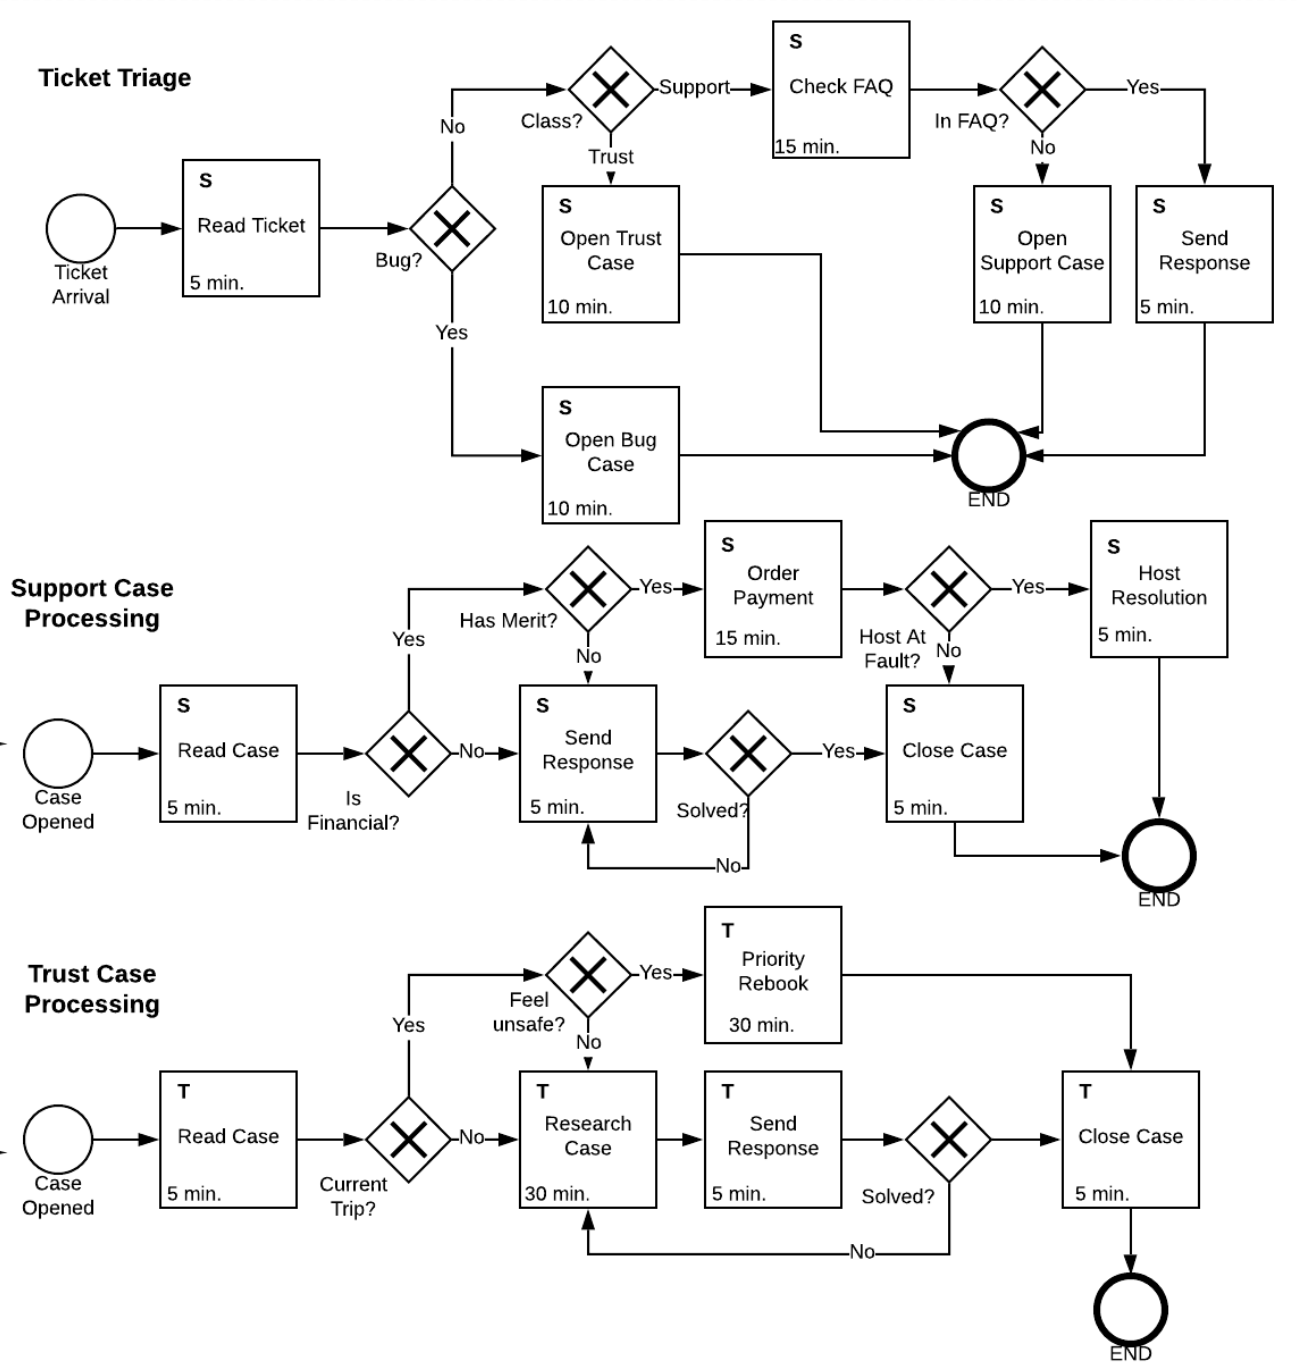
\includegraphics[width=0.8\textwidth]{tex/workflows.png}
  \caption{Customer support workflows, enacted to generate logs}
  \label{fig:workflows}
\end{figure}

\begin{figure}[h!]
  \centering
  \begin{footnotesize}
  \begin{tabular}{|c|c|c|l|l|}\hline
batch               & timestamp     & enactment id  & event type                    & event data                              \\\hline
\multirow{10}{*}{42} & 42             & $\mu_{1}$     & \texttt{ReadCase}            & \{ name=Alice, support=1 \}             \\\cline{2-5}
                    & 42             & $\mu_{1}$     &  \texttt{SendResponse}        & \{ name=Alice \}                        \\\cline{2-5}
                    & 42             & $\mu_{2}$     &  \texttt{ReadCase}            & \{ name=Bob, support=2 \}               \\\cline{2-5}
                    & 42             & $\mu_{1}$     &  \texttt{SendResponse}        & \{ name=Alice \}                        \\\cline{2-5}
                    & 42             & $\mu_{2}$     &  \texttt{SendResponse}        & \{ name=Bob \}                          \\\cline{2-5}
                    & 42             & $\mu_{2}$     &  \texttt{CloseCase}           & \{ name=Bob, support=2 \}               \\\cline{2-5}
                    & 42             & $\mu_{1}$     &  \texttt{CloseCase}           & \{ name=Alice, support=1 \}             \\\cline{2-5}
                    & 42             & $\mu_{3}$     &  \texttt{ReadCase}            & \{ name=David, support=2\}              \\\cline{2-5}
                    & 42             & $\mu_{4}$     &  \texttt{ReadCase}            & \{ name=Charlie, support=1 \}           \\\cline{2-5}
                    & 42             & $\mu_{4}$     &  \texttt{OrderPayment}        & \{ name=Charlie \}                      \\\cline{1-5}
\multirow{3}{*}{43}  & 43             & $\mu_{3}$     &  \texttt{SendResponse}        & \{ name=David \}                        \\\cline{2-5}
                    & 43             & $\mu_{4}$     &  \texttt{SendResponse}        & \{ name=Charlie \}                      \\\cline{2-5}
                    & \dots         & \dots         & \dots                         & \dots                                   \\\hline
    \end{tabular}
  \end{footnotesize}
  \caption{Portion of a log with {\sc support case} enactments with ten events per batch}
  \label{fig:log}
\end{figure}

We generated rules using the workflows' activities, e.g., 
\texttt{ReadCase}, \texttt{SendResponse}, etc.,
and gap atoms with one- to ten-second gaps,
reflecting the typical gaps between events in enactments.
We respect the workflow model's activity ordering
to ensure gap atoms are satisfiable
by some enactments.
We use two classes of rules: ``small'' and ``medium'' rules,
as shown in Figure\:\ref{fig:sample-rules}.
For {\em small} rules,
each rule body has one or two event atoms and no more than one gap,
and each rule head has one event and no more than one gap.
For {\em medium} rules,
each rule body has up to two event atoms and no more than two gaps
and each rule head has up to two event atoms and no more than two gaps.
We also categorize sets of rules by their ``overlap'',
defined in Section\:\ref{subsec:rule-properties}
to approximate the potential for rule interaction.

\begin{figure}[h!]
  \begin{tabular}{lcl}
    \multicolumn{3}{c}{Small rules (2 to 4 atoms), overlap of $0.33$}\\
    $r_1: \texttt{ReadCase}(u,i)@x$                                           & $\rightarrow$ & $\texttt{SendResponse}(u)@y, y {\leq} x + 5$ \\
    $r_2: \texttt{ReadCase}(u,i)@x, \texttt{SendResponse}(u)@y,$              & $\rightarrow$ & $x+10 {\leq} y$ \\
    $r_3: \texttt{ReadCase}(u,i)@x, \texttt{OrderPayment}(u)@y,$              & $\rightarrow$ & $y {\leq} x + 3, \texttt{CloseCase}(u,i)@z$ \\
    \multicolumn{3}{c}{}\\
    \multicolumn{3}{c}{Medium rules (5 to 7 atoms), overlap of $0.66$}\\
    $r_4: \texttt{ReadCase}(u,i)@x$                                             & $\rightarrow$ & $\texttt{SendResponse}(u)@y, x + 3 \leq y$ \\
                                                                                &               & $\texttt{CloseCase}(u,i)@z, z {\leq} x + 5, z {\leq} y + 1$ \\
    $r_5: \texttt{ReadCase}(u,i)@x, \texttt{SendResponse}(u)@y,$   & $\rightarrow$ & $\texttt{CloseCase}(u,i)@z, z {\leq} x + 5, z {\leq} y + 1$ \\
    \hspace{0.5cm}$x + 4 {\leq} y$                                 &               & \\
    $r_6: \texttt{ReadCase}(u,i)@x, \texttt{OrderPayment}(u)@y,$  & $\rightarrow$ & $\texttt{HostResolution}(u)@w, x + 10 {\leq} w$\\
    \hspace{0.5cm}$x + 10 \leq y$                                 &              & $y {\leq} w + 10$ \\ 
  \end{tabular}
  \caption{Sample small and medium-sized rules}
  \label{fig:sample-rules}
\end{figure}

Experiments were run on a single machine:
a desktop Fedora 20 (Linux) machine
with a 2K MHz, 8-core AMD EPYC 7702 processor with 8GB memory.
The implementation was written in Python 3.9.6.
We used the Z3 SMT solver \cite{de2008z3} for satisfiability checking
and the Python bindings for Z3 \cite{z3py}.
Notably,
in early implementations of the monitor,
we invoked the Z3 library many times to instantiate each subformula,
then combined these subformula for the satisfiability test
with z3.Solver.check.
The multiple library calls resulted in much slower processing,
up to $100$ times as long as our reported results;
a frugal use of the solver is critical
to achieve reasonable performance.
The source code of the monitor
and experimental framework is available on Github
\cite{mackeymultirulemonitor}.

\subsection{Detection Often Occurs Far Before Enactments End}
\label{subsec:earliness}

First, we examine how early
violations are detected
with respect to enactments' events.
The quantification of earliness
indicates potential benefits
where the earliness affects the system's response.
For example,
the system may choose to halt an enactment
when a violation is detected,
allowing the system to reclaim resources
or to prevent further policy violations.
We report the average earliness of violation detection
for the single-rule monitor
with respect to the enactment's length.
Because the multi-rule monitoring algorithm
is an extension of the single-rule algorithm
and can detect some violations earlier,
the earliness afforded by multi-rule monitoring
is at least as good as that of single-rule monitoring
and may be better in some cases.

We apply the single-rule monitor
to logs with normal-length ($\approx$10 events)
and large enactments ($\approx$100 events).
For each enactment, we count the observed events after the first
detected violation.
Fig.\,\ref{fig:eval_early_detection_benefits} shows that,
on average, violations are detected at 75\% of
event arrival for normal-length enactments and 34\% for large ones.
As detailed in Section \ref{sec:motiv},
this happens when expected head event atoms are pending,
but their timestamps are bounded by body event atoms
and some gap atoms.
Often,
the upper bound timestamp of a head event atom falls within the enactment's duration,
leading {\sf Detect} to recognize its occurrence in real-time.
We focus on average earliness for single-rule monitoring,
but the multi-rule approach often detects even earlier,
as shown in Section\:\ref{sec:multiple}.
Finally, we note that the average earliness
is affected by the gaps in gap atoms;
more study is needed to understand the relationship
between gap size and average earliness. 

\begin{figure}[ht]
  \vspace{-2mm}
  \centering
  \begin{footnotesize}
    \renewcommand{\arraystretch}{1.6}
  \begin{tabular}[t]{|c||c|c||c|c|}\cline{2-5}
   \multicolumn{1}{c}{}         & \multicolumn{2}{|c||}{\bf Normal-length enactments}          & \multicolumn{2}{|c|}{\bf Large enactments}  \\\hline
    {\bf Rule Size}   & \% events before first violation  & \% after & \% events before first violation  & \% after \\\hline
    {\bf Small}  & 74.9 & 25.1  & 33.5 & 66.5                 \\\hline
    {\bf Medium} & 83.7 & 16.3  & 69.4 & 30.6              \\\hline
  \end{tabular}
  \end{footnotesize}
  \caption{Percentages of events observed before and after the first detected violation}
  \vspace*{-2mm}
  \label{fig:eval_early_detection_benefits}
\end{figure}

\subsection{Detection is Feasible for Medium-scale Applications}
\label{subsec:log-properties}

Next,
we study the feasibility of monitoring.
We evaluate when the monitor
processes batches
in an average of less than one second,
the batch arrival rate.
The batch size and the enactment concurrency
determine the number of assignments
that must be joined and matched
in the {\sf Update} and {\sf Update-E} algorithms,
the number of expected events generated by the {\sf Chase} algorithm,
and the number of matches that contribute 
to the formula produced by {\sf Build},
so we expect that increasing these parameters raises the processing time.

First, we report the average processing time
for the single-rule monitor (Section \ref{sec:alg})
in Figure\:\ref{fig:eval_avg_proc_time}.
The average processing time is far less than one second
for all batch sizes and enactment lengths,
shorter than $0.07$ seconds for all small rules and 
shorter than $0.2$ seconds for all medium rules,
indicating that the single-rule monitor is feasible
for logs with those properties.
These times increase linearly with the batch size,
which is expected for small rules,
as the number of possible assignments
does not yet suffer the combinatorial explosion.
For medium rules, however,
the average processing time also increases linearly
with the batch size;
this is unexpected because
to make the number of assignments
is exponential in the batch size.
This may be due to the increasing number of gap atoms,
as more gap atoms decrease
the number of assignments in the body or head table.
This phenomenon requires a more thorough investigation
of the effects of gap atoms on the assignment database.

\begin{figure}[ht]
  {
    \centering
    \begin{footnotesize}
      \renewcommand{\arraystretch}{1.6}
    \begin{tabular}[t]{|c||c|c||c|c||}\cline{2-5}
    \multicolumn{1}{c}{}& \multicolumn{4}{|c|}{\bf Enactment Length}\\\cline{2-5}
    \multicolumn{1}{c}{} & \multicolumn{1}{|c|}{\bf Normal}
    & \multicolumn{1}{|c||}{\bf Large} 
    & \multicolumn{1}{|c|}{\bf Normal}
    & \multicolumn{1}{|c|}{\bf Large} \\\hline
    {\bf Batch Size} & \multicolumn{2}{|c||}{{\bf Small Rules}} & \multicolumn{2}{|c||}{{\bf Medium Rules}}\\\hline\hline
    100             & 4.55$\times10^{-4}$     & 6.19$\times10^{-4}$     & 7.74$\times10^{-4}$     & 1.363$\times10^{-3}$     \\\hline
    1,000           & 4.330$\times10^{-3}$    & 6.177$\times10^{-3}$    & 7.534$\times10^{-3}$    & 1.3509$\times10^{-2}$     \\\hline
    10,000          & 4.2414$\times10^{-2}$   & 6.0769$\times10^{-2}$   & 7.4925$\times10^{-2}$   & 1.35218$\times10^{-1}$     \\\hline
    \end{tabular}
  \end{footnotesize}
    \vspace*{-2mm}
    \caption{Batch Processing Times (seconds) by Batch Size, Rule Size, and Enactment Length}
    \label{fig:eval_avg_proc_time}
    }
  \end{figure}

We also evaluated the feasibility of the multiple-rule monitor.
We monitored logs with normal-length enactments
and rule sets with three medium rules
with an average overlap of one event atom.
The results in Table \ref{tab:experiment-log-properties} show
the batch processing time increases with the batch size and concurrency
as expected.
Second,
the average processing time is ${\le}1$ second
for batches of $100$ events and an average enactment concurrency of $100$.
Beyond these values,
the average processing time exceeds ${\ge}1$ second,
shown by parentheses in the table,
but is still ${\le}10$ seconds.

We note here that 
our experiments were conducted on a single commodity machine
rather than enterprise-grade hardware;
our results suggest that
multi-rule monitoring would be feasible
for a wider range of applications,
i.e., larger batches and more concurrent enactments,
if the monitoring is performed with more powerful hardware resources.

\begin{table}[htbp]
    \centering
    \begin{footnotesize}
  \begin{tabular}{|c|c|c|c|c|c|}
  \hline
  \textbf{Batch Size} & \textbf{Conc=10} & \textbf{Conc=50} & \textbf{Conc=100}  & \textbf{Conc=500}  & \textbf{Conc=1,000} \\\hline\hline
  10                  & 0.061            & 0.046            & 0.294              & (1.253)              & (3.031)               \\\hline
  50                  & 0.195            & 0.169            & 0.403              & (2.506)              & (3.269)               \\\hline
  100                 & 0.374            & 0.328            & 0.553              & (2.807)              & (3.483)               \\\hline
  500                 & (1.256)          & (1.851)          & (1.326)            & (3.347)              & (5.279)               \\\hline
  \hline
  \end{tabular}
\end{footnotesize}
  \caption{Average Batch Processing Time (seconds) by Batch Size and Concurrency}
  \label{tab:experiment-log-properties}
\end{table}

\subsection{Detection Remains Feasible for Complex Sets of Rules}
\label{subsec:rule-properties}

Another factor affecting the feasibility of monitoring
is the size and ``overlap'' the sets of rules.
The {\em overlap} for a set of rules
is the number of pairs of event atoms
that share the same name
such that one appears in the head of one rule
and the other appears in the body of another rule,
divided by the total number of rule pairs.
More overlap between rules increases the number of assignments
generated by expected events from the {\sf Chase} algorithm,
thus increasing the number of assignments to process into
the assignment database by {\sf Update} and {\sf Update-E}.
Furthermore,
expected events can create more expected events
in the subsequent executions of the {\sf Chase} algorithm's
{\bf while} loop,
but this feedback is ultimately limited by the acyclicity
of the rule set.
Finally,
expected events carry marked nulls,
which are added to the formula produced by {\sf Build},
so more overlap grows the subformula in the formula
that share variables;
this may increase the time to check its satisfiability.

We used logs with batches of one hundred events
and an average of one hundred concurrent enactments,
as these values were found to be within the feasible range
for the multi-rule monitor
in Section\:\ref{subsec:log-properties}.
We generated thirty sets
with two to four small rules,
calculating the overlap by summing the overlap
for each pair of rules,
then dividing by the number of rule pairs.
We place each rule in one of five categories:
$0.33$, $0.66$, $1$, $1.33$, and $1.66$ event atoms,
whichever is closest to its average overlap.
In Table\:\ref{tab:overlap-experiment}, 
we report the average batch processing time
with any time above the batch arrival rate of one second
shown in parentheses to indicate infeasibility.
the overlap grows exponential as the overlap increases linearly.
Furthermore,
we see when the average overlap
exceeds $1$ event atom per rule pair,
the processing time exceeds one second,
the threshold for feasibility.

\begin{table}[htbp]
  \centering
\begin{tabular}{|c|c|c|c|c|}
\hline
\textbf{Overlap$\approx$0.33}  & \textbf{Overlap$\approx$0.66} & \textbf{Overlap$\approx$1} & \textbf{Overlap$\approx$1.33} & \textbf{Overlap$\approx$1.66} \\\hline\hline
0.048                  & 0.169                 & 0.356              & (1.22)                  & (3.17)                  \\\hline
\end{tabular}
\caption{Average Batch Processing Time (seconds) by Average Overlap}
\label{tab:overlap-experiment}
\end{table}

We also evaluated the effect of varying the number of rules
while keeping a constant overlap.
More rules grows the number of tables and entries
in the assignment databases,
as well as the number of expected events
generated by the {\sf Chase},
as each rule's body assignment generates expected events.
The average overlap for the sets of rules was $0.54$,
so we used five rule sets of two, three, four, and five small rules
with an overlap of $0.54 \pm 0.2$.
We report the average batch processing times
in Table\:\ref{tab:number-rules-experiment}.
The batch processing time increases
exponentially with the number of rules;
this suggests the number of rules
is similarly critical to the feasibility of monitoring
as the overlap,
where rule sets with relatively low overlap
can become infeasible
when the number of rules exceeds four.

\begin{table}[htbp]
  \centering
\begin{tabular}{|c|c|c|c|}
\hline
\textbf{2 rules} & \textbf{3 rules} & \textbf{4 rules} & \textbf{5 rules} \\\hline\hline
0.014                  & 0.099      & 0.395            & (1.582)            \\\hline
\end{tabular}
\caption{Average Batch Processing Time (seconds) for Overlap${\approx}0.54$ by Number of Rules}
\label{tab:number-rules-experiment}
\end{table}

In summary, our evaluation
quantifies
the benefits of early violation detection
and the feasibility of monitoring
with respect to the size and complexity of logs and rules.
We identify the algorithms and subroutines 
that are most affected by these dimensions
and provide explanations for the observed trends.
We also identify dimensions of logs and rules
that deserve further investigation,
such as the effects of gap size on earliness
and the effects of gap size and number of gaps on processing time.
Finally,
we note that these findings are limited 
to applications with similar characteristics as the sample logs
and rules we used in our evaluation,
and thus may not generalize to arbitrary event-based systems.
More work is needed to extend these findings to a wider range of applications,
particularly by testing real-world logs and rules.

\section{Related Work}
\label{sec:early-violation-detection-related-work}

We first discuss related work that reasons algorithmically
about when a violation is inevitable.
Then, we compare our work with other approaches
that monitor constraints with data values.

A key technique in this work
is to detect violations at the earliest possible time.
References \cite{maggi2011monitoringcolored,maggi2012runtime,
maggi2011runtime} studies violations
of constraints in {\sc declare} language,
using
an encoding of violations' temporary or permanent status in states of automata.
Quantitative time constraints,
such as ``for every request followed within five days by a response,
a payment is made within three days of the response and three days of the request'',
are important
for applications of runtime monitoring \cite{ly2015compliance},
but difficult to encode in automata,
as evidenced by the previous chapter.
We identify violations
as inevitable or not
by partially instantiating constraints
with observed timestamps and data values
and checking satisfiability of the resulting constraints.
References \cite{dousson2007chronicle} and \cite{maggi2019compliance}
also partially initialize
constraints to detect violations,
but do not consider interactions between sets of constraints,
which may produce earlier violations as illustrated above.

Another functionality of runtime constraints
considered by this chapter
is the comparison of data values,
such as matching the user who makes a request
to the user who receives a response.
References \cite{de2013runtime,riccardo2014monitoringfsa}
monitor constraints in first-order LTL
with automata whose states have relational data stores,
though they assume a fixed, finite domain of data values,
which is impractical for large applications.
Quantified event automata, finite-state automata
with transitions labeled by quantified first-order formulas,
can also monitor data-dependent constraints
\cite{barringer2012quantified}.
Their approach creates and manages bindings to variables,
but is limited by the same drawbacks as
automata-based approaches described above.
Other work on first-order LTL uses exclusively relational data structures
as auxillary storage for violation detection
\cite{Chomicki95:TODS,halle2012runtime,basin2015monitoring,havelund2018efficient},
though they do not calculate deadlines explicitly
because they do not use quantitative time constraints.
Also relevant is the technique of trace slicing
\cite{chen2009parametric},
filtering an enactment
into disjoint enactments with related data,
allowing multiple monitors to run in parallel.
Our work does not use trace slicing,
but it seems promising for optimization
as a pre-processing step
to parallelize our approach.

% References \cite{, cimatti2020smt, havelund2018efficient, calvanese2022verification}

Other relevant data-centric approaches
are those for relational databases and Datalog rules.
Incremental view maintenance
for Datalog provides incremental algorithms
for updating the results of views or queries
when the underlying database changes;
\cite{gupta1993maintaining} maintains
Datalog and SQL views
without gap constraints
nor existential variables and multiple atoms in the rule head.
A key technique in this work comes from the observation that
because we use Datalog-like rules,
the possibility of rules triggering other rules
can be simulated by the chase \cite{AHV95},
which we adapt for our setting in Section\:\ref{sec:multiple}.
Other work on the chase
for Datalog with arithmetic constraints
targets problems that don't apply to our setting
of monitoring an enactment at runtime,
including computing certain query answers \cite{afrati2008data, ten2013data}.

\section{Chapter Summary}
\label{sec:rules-data-conclusion}

This chapter presents techniques for detecting violations
of individual rules and sets of rules with data,
extending the class of rules that can be monitored.
We showed that detecting violations at the earliest possible time.
can be accomplished by reasoning about timestamps,
simulating rule interaction,
and applying satisfiability testing to potential violations.
We also conducted an empirical evaluation of our techniques
to show that they are effective and efficient
for small- and medium-sized batches
and rules,
though more study is needed
to determine their effectiveness and efficiency
with enterprise-scale computing resources.
In the next chapter,
we explore the use of aggregation functions
over time windows in rules.